% This is "sig-alternate.tex" V2.0 May 2012
% This file should be compiled with V2.5 of "sig-alternate.cls" May 2012
%
% This example file demonstrates the use of the 'sig-alternate.cls'
% V2.5 LaTeX2e document class file. It is for those submitting
% articles to ACM Conference Proceedings WHO DO NOT WISH TO
% STRICTLY ADHERE TO THE SIGS (PUBS-BOARD-ENDORSED) STYLE.
% The 'sig-alternate.cls' file will produce a similar-looking,
% albeit, 'tighter' paper resulting in, invariably, fewer pages.
%
% ----------------------------------------------------------------------------------------------------------------
% This .tex file (and associated .cls V2.5) produces:
%       1) The Permission Statement
%       2) The Conference (location) Info information
%       3) The Copyright Line with ACM data
%       4) NO page numbers
%
% as against the acm_proc_article-sp.cls file which
% DOES NOT produce 1) thru' 3) above.
%
% Using 'sig-alternate.cls' you have control, however, from within
% the source .tex file, over both the CopyrightYear
% (defaulted to 200X) and the ACM Copyright Data
% (defaulted to X-XXXXX-XX-X/XX/XX).
% e.g.
% \CopyrightYear{2007} will cause 2007 to appear in the copyright line.
% \crdata{0-12345-67-8/90/12} will cause 0-12345-67-8/90/12 to appear in the copyright line.
%
% ---------------------------------------------------------------------------------------------------------------
% This .tex source is an example which *does* use
% the .bib file (from which the .bbl file % is produced).
% REMEMBER HOWEVER: After having produced the .bbl file,
% and prior to final submission, you *NEED* to 'insert'
% your .bbl file into your source .tex file so as to provide
% ONE 'self-contained' source file.
%
% ================= IF YOU HAVE QUESTIONS =======================
% Questions regarding the SIGS styles, SIGS policies and
% procedures, Conferences etc. should be sent to
% Adrienne Griscti (griscti@acm.org)
%
% Technical questions _only_ to
% Gerald Murray (murray@hq.acm.org)
% ===============================================================
%
% For tracking purposes - this is V2.0 - May 2012

\documentclass{sig-alternate}
\usepackage[latin1]{inputenc}
\usepackage{graphicx}        % standard LaTeX graphics tool
\usepackage{subfigure}
\usepackage{url}


\begin{document}
%
% --- Author Metadata here ---
\conferenceinfo{GECCO'13,} {July 6-10, 2013, Amsterdam, The Netherlands.}
    \CopyrightYear{2013}
    \crdata{TBA}
    \clubpenalty=10000
    \widowpenalty = 10000

\title{Migration study on a Pareto-based island model for MOACOs}

%\subtitle{[Extended Abstract]
%\titlenote{A full version of this paper is available as
%\textit{Author's Guide to Preparing ACM SIG Proceedings Using
%\LaTeX$2_\epsilon$\ and BibTeX} at
%\texttt{www.acm.org/eaddress.htm}}}
%
% You need the command \numberofauthors to handle the 'placement
% and alignment' of the authors beneath the title.
%
% For aesthetic reasons, we recommend 'three authors at a time'
% i.e. three 'name/affiliation blocks' be placed beneath the title.
%
% NOTE: You are NOT restricted in how many 'rows' of
% "name/affiliations" may appear. We just ask that you restrict
% the number of 'columns' to three.
%
% Because of the available 'opening page real-estate'
% we ask you to refrain from putting more than six authors
% (two rows with three columns) beneath the article title.
% More than six makes the first-page appear very cluttered indeed.
%
% Use the \alignauthor commands to handle the names
% and affiliations for an 'aesthetic maximum' of six authors.
% Add names, affiliations, addresses for
% the seventh etc. author(s) as the argument for the
% \additionalauthors command.
% These 'additional authors' will be output/set for you
% without further effort on your part as the last section in
% the body of your article BEFORE References or any Appendices.


\numberofauthors{2}
 \author{
 \alignauthor
 Jack, Sawyer, Hurley\\
        \affaddr{Lost island}\\
        \affaddr{Unknown}\\
        \affaddr{Pacific Ocean}\\
        \email{jack,sawyer,hurley@lost.com}
 \alignauthor
 Locke\\
 \affaddr{Lost island}\\
 \affaddr{Unknown}\\
 \affaddr{Pacific Ocean}\\
 \email{locke@lost.com}
 }

%\numberofauthors{2}
% \author{
% \alignauthor
% J.J. Merelo, A.M. Mora, C. M. Fernandes\\
%        \affaddr{University of Granada}\\
%        \affaddr{Department of Computer Architecture and Technology, ETSIIT}\\
%        \affaddr{18071 - Granada}\\
%        \email{jmerelo,amorag,cfernandes@geneura.ugr.es}
% \alignauthor
% Anna I. Esparcia-Alc�zar\\
% \affaddr{S2 Grupo}\\
% \email{aesparcia@s2grupo.es}
% }


%\numberofauthors{4} %  in this sample file, there are a *total*
% of EIGHT authors. SIX appear on the 'first-page' (for formatting
% reasons) and the remaining two appear in the \additionalauthors section.
%

%\author{
% You can go ahead and credit any number of authors here,
% e.g. one 'row of three' or two rows (consisting of one row of three
% and a second row of one, two or three).
%
% The command \alignauthor (no curly braces needed) should
% precede each author name, affiliation/snail-mail address and
% e-mail address. Additionally, tag each line of
% affiliation/address with \affaddr, and tag the
% e-mail address with \email.
%
% 1st. author
%\alignauthor
%Jack\\
%       \affaddr{Lost island}\\
%       \affaddr{unknow}\\
%       \affaddr{Pacific Ocean}\\
%       \email{jack_the_doctor@lost.com}
% 2nd. author
%\alignauthor
%Sawyer\\
%       \affaddr{Lost island}\\
%       \affaddr{unknow}\\
%       \affaddr{Pacific Ocean}\\
%       \email{sawyer_tom@lost.com}
% 3rd. author
%\alignauthor 
%Lock\\
%       \affaddr{Lost island}\\
%       \affaddr{unknow}\\
%       \affaddr{Pacific Ocean}\\
%       \email{lock@lost.com}
% 4rd. author
%\alignauthor 
%Hurley\\
%       \affaddr{Lost island}\\
%       \affaddr{unknow}\\
%       \affaddr{Pacific Ocean}\\
%       \email{hugo@lost.com}
%}

%\and  % use '\and' if you need 'another row' of author names
% 4th. author
%\alignauthor Lawrence P. Leipuner\\
%       \affaddr{Brookhaven Laboratories}\\
%       \affaddr{Brookhaven National Lab}\\
%       \affaddr{P.O. Box 5000}\\
%       \email{lleipuner@researchlabs.org}
% 5th. author
%\alignauthor Sean Fogarty\\
%       \affaddr{NASA Ames Research Center}\\
%       \affaddr{Moffett Field}\\
%       \affaddr{California 94035}\\
%       \email{fogartys@amesres.org}
% 6th. author
%\alignauthor Charles Palmer\\
%       \affaddr{Palmer Research Laboratories}\\
%       \affaddr{8600 Datapoint Drive}\\
%       \affaddr{San Antonio, Texas 78229}\\
%       \email{cpalmer@prl.com}
%}
% There's nothing stopping you putting the seventh, eighth, etc.
% author on the opening page (as the 'third row') but we ask,
% for aesthetic reasons that you place these 'additional authors'
% in the \additional authors block, viz.
%\additionalauthors{Additional authors: John Smith (The Th{\o}rv{\"a}ld Group,
%email: {\texttt{jsmith@affiliation.org}}) and Julius P.~Kumquat
%(The Kumquat Consortium, email: {\texttt{jpkumquat@consortium.net}}).}
%\date{30 July 1999}
% Just remember to make sure that the TOTAL number of authors
% is the number that will appear on the first page PLUS the
% number that will appear in the \additionalauthors section.

\maketitle

\begin{abstract}
Pareto-based island model is a multi-colony distribution scheme recently presented for the resolution, by means of ant colony optimization algorithms, of bi-criteria problems. It yielded very promising results, but the model was implemented considering a unique Pareto-front-shaped unidirectional neighborhood migration topology, and a constant migration rate.
In the present work two additional neighborhood topology schemes, and four different migration rates have been tested, considering the algorithm which obtained the best results in average in the model presentation article: MOACS (Multi-Objective Ant Colony System).
Several experiments have been conducted, including statistical tests for better support the study. 
High values for the migration rate and the use of a bidirectional neighborhood migration topology yields the best results.
\end{abstract}

% A category with the (minimum) three required fields
\category{H.4}{Information Systems Applications}{Miscellaneous}
%A category including the fourth, optional field follows...
\category{G.1.6}{Mathematics of Computing}{Numerical Analysis}[Optimization]

% Antonio - A ver si te mola esta categor�a tambi�n:
%D.2.8 [Software Engineering]: Metrics�complexity mea-
%sures, performance measures
\terms{Algorithms}
% Antonio - no se si se puede a�adir alg�n otro t�rmino (Theory?)

\keywords{Multi-objective ant colony optimization algorithms, MOACO, ACO, multi-colony, distributed algorithms, island model, migration rate, neighborhood migration topology}


%
%%%%%%%%%%%%%%%%%%%%%%%%%%%%%%%   INTRODUCTION   %%%%%%%%%%%%%%%%%%%%%%%%%%%%%%%
%
\section{Introduction}
\label{sec:intro}
%

Island model is one of the most extended distribution paradigms, since it arose in the Evolutionary Algorithms (EA) scope \cite{GA_Island_Model}. It proposed the division of the whole population into different subpopulations called islands. They evolve independently a number of generations and then, some individuals (normally the best) migrate between them. Thus, the optimization process is improved due to the parallel exploration of different areas of the search space that every island is focused on, and in addition, thanks to the inclusion of different promising individuals in a population, which guides the search and probably avoids local optima stagnation. Moreover, the distribution means an inherent running time improvement.
There are several factors to consider in an island model, such as the migration rate (number of times the individuals are moved between islands), the neighborhood topology (island connections) or the replacement policy (which individuals are removed of the receiver population to include the migrants).

This model was initially proposed for the resolution of problems with just one objective, but it was later adapted to solve multi-objective problems \cite{Osyczka1985}.
Multi-objective optimization problems (MOPs) are those where more than one independent function must be optimized at once, every function is an objective and the improvement of one does not mean an improvement in the rest. There is a set of the so-called non-dominated solutions (those which better satisfy each of the functions) rather than just one, which constitutes the Pareto set (PS). The graphical representation of this Pareto-optimal set of solutions is named the Pareto front (PF).
Thus, the main issue of a good multi-objective (MO) algorithm
\cite{Coello2002} is to obtain the maximum number of non-dominated solutions, having a high diversity and spread, and being as closer to the optimal set as possible.

In addition to EAs, Ant colony optimization (ACO) is another metaheuristic well-suited for distribution. ACO \cite{ACO_2003} algorithms are based in the behaviour of natural ants when searching for food, and the way they build shortest paths between their nest and any interesting point. This behaviour has been explained through the concept of \textit{stigmergy}, that is, communication using the environment, so every ant, while walking, deposits on the ground a chemical substance called \textit{pheromone} which the others can smell (and which is evaporated after some time). One ant tends to follow strong concentrations of pheromone caused by repeated passes of ants; a pheromone trail is then formed from nest to food source, so in intersections between several trails an ant moves with high probability following the highest pheromone level.

Ants are modelled as a set of artificial agents which search in a weighted graph for the optimal paths. These agents cooperate to explore the search space and to build the solution for a problem.
The ACOs adapted to the resolution of problems with several objectives are known as multi-objective ant colony optimization algorithms or MOACOs. 

As stated, ACO algorithms can be directly parallelized due to the inherent independent work of the ants. Thus, several parallel ACO approaches have been proposed since the metaheuristic was presented \cite{Survey_par_ACOs}, most of them devoted to address specific problems. %\cite{ParallelACO_TSP,ParallelAS_CVRP,ParallelACO_MTTP}.

There are two main distribution levels: coarse-grained (parallelization at colony level) \cite{ParallelACO_MultiColony}, and fine-grained (parallelization at ant level) \cite{ParallelACO_FineGrained}. The first approach is the most extended and is known as multi-colony model, since the ants are divided in sub-colonies which can operate independently from the rest \cite{ParallelACO_CoarseGrained_T} or can share any information (pheromone trails for instance) \cite{ParallelACO_CoarseGrained_B}.

In this line, there was proposed in a recent paper a multi-colony distribution model named \textit{Pareto-based island model} \cite{iMOACOS_SOCO}, which spread the ants, grouped in colonies, into several computational nodes (processors in clusters) or islands. Everyone focuses on a different area of the search space, promoting the exploration and finally yielding a better set of results than a mono-colony standard approach. Thus, a bigger amount of non-dominated solutions, with higher quality (closer to the optimal values), and with a better spread or distribution over the ideal set of solutions were obtained. To this end, some migrations were performed between the colonies (moving ants/solutions), increasing the explorative component which turns on getting a better performance. This model defined a neighborhood topology based on the
Pareto front form and was compared with two other methods based in independent \textit{multi-colony} structures.
The proposed island model, based in the Pareto front, obtained excellent results in the comparison with the other models (multi-start and independent multi-colonies). All of them were implemented as substrates for three different MOACOs from the literature: Iredi's et al. \textit{BIANT} \cite{BiANT-Iredi}, Bar�n's et al. \textit{MOACS} \cite{MOACS-Baran}; and an algorithm named \textit{CHAC} \cite{CHAC_COR}. MOACS and CHAC yielded the best results, very similar between them. But since it was an initial proof of concept, the island model just implemented a neighborhood topology (unidirectional) and was tested with just a migration rate value (every 50 iterations).

There are just a few papers studying island models in ACOs scope \cite{ParallelACO_Island,ParallelACO_Island_Topologies}, but to our best knowledge, just the works \cite{iMOACOs_IWANN,iMOACOS_SOCO} involve the distribution of MOACOs following an island-model shape.

Thus in the present work a deeper analysis of the Pareto-based island model is proposed. Three different neighborhood topologies will be tested: \textit{unidirectional}, \textit{bidirectional} and \textit{broadcast}; along with four different migration rates: every 25, 50, 75 and 100 iterations. Due to space limitations, just MOACS algorithm will be considered, according to the good performance it presented in previous papers.
The results, including different metrics, obtained with every configuration solving the \textit{Symmetric Bi-criteria Travelling Salesman Problem} (bTSP), will be analyzed by means of statistical tools, such as the Analysis of variance (ANOVA) \cite{ANOVA_Fisher} and post-hoc Tukey's Honestly Significant Difference tests (Tukey HSD) \cite{Tukey_HSD}.

%The rest of the paper is structured as follows: the next section briefly introduces multi-objective optimization concepts which are dealt in the work.
%The algorithm to analyse, MOACS, is described in Section \ref{sec:moacs}. Then, Section \ref{sec:PB_island_model} introduces the distributed Pareto-based island model to study and presents the different neighborhood topologies to test. 
%The conducted experiments are presented in Section \ref{sec:experiments}, along with the analysis of the results. Finally, conclusions and future lines of work are commented in Section \ref{sec:conclusions}.


%%%%%%%%%%%%%%%%%%%%%%%%%%%%  MO Optimization  %%%%%%%%%%%%%%%%%%%%%%%%%%%%%%%%

\section{Multi-objective optimization}
\label{sec:mulobj}

Multi-Criteria or Multi-Objective Optimization Problems\\ (MOP)
\cite{Osyczka1985} are those where several 
 objectives have to be simultaneously optimized. These problems do not
 have a single best solution, one that is better than any other with
 respect to every objective. In fact, frequently improving the
 solution for one objective implies a worsening for another. 
%
Thus in a MOP there is a set of solutions that are better than the rest considering all the objectives; this set is known as the \textit{Pareto set} (PS). They try to approach the ideal set of solutions
which is usually represented graphically as the \textit{Pareto front} (PF). These are related to an important concept, the \textit{dominance}, defined as follows (\textit{a} dominates \textit{b}):
%
\begin{small}
\begin{equation}\label{eq:modom}
\begin{array}{ll}
a \prec b\;\;if: \\
\forall i\in 1,2,...,k \; | \; C_i(a)\leq C_i(b)\:\; \wedge \:\; \exists j\in 1,2,...k \;| \; C_j(a)<C_j(b)
\end{array}
\end{equation}
\end{small}
%
where \textit{a $\in$ X} and \textit{b $\in$ X} are two different decision vectors of \textit{n} values, and every \textit{C} is a cost function (one per objective). If it intends to minimize the cost and Equation \ref{eq:modom} is true, then \textit{b is dominated by a}.

Hence, the solutions in the PS are known as \textit{non-dominated solutions}, while the remainder are known as dominated solutions. 
%
%Figure \ref{fig:pareto_front} shows the representation of the PF of a multi-objective (bi-criteria) problem, where the domination concept can be clearly seen.
%
%\begin{figure}[ht]
%\begin{center}
%\includegraphics[scale=0.5]{figures/pareto_front.eps}
%\caption{Example of the Pareto front in a problem with two objectives to minimize (F1 and F2). Black dots correspond to solutions in the Pareto front ($a$ and $b$ among them). Dominated solutions are shown in gray ($c$ for instance).
%\label{fig:pareto_front}}
%\end{center}
%\end{figure}
%
Since none of the solutions in the PS is absolutely better
than the other non-dominated solutions, all of them are equally
acceptable as regards the satisfaction of all the objectives. These concepts can be extended in \cite{Coello2002}. 


%%%%%%%%%%%%%%%%%%%%%%%%%%%%%%  MOACO TO STUDY  %%%%%%%%%%%%%%%%%%%%%%%%%%%%%%
%
\section{MOACS algorithm}
\label{sec:moacs}

The algorithm to study is the well-known {\em MOACS} (Multi-Objective Ant Colony System), which was proposed by Bar�n et al.~\cite{MOACS-Baran}, to solve the Vehicle Routing Problem with Time Windows (VRPTW), a bi-objective problem. The good results it yielded in the article \cite{iMOACOS_SOCO}, where the Pareto-based island model was presented and tested, is the reason why it has been chosen as the algorithm to study in the present work.

As main features it considers a single pheromone matrix for both objectives, and follows a State Transition Rule (STR), for building the solutions, described as:\\
\\
\begin{small}
If (\textit{q} $\le$ \textit{q}$_{0}$)
%
\begin{equation} \label{eq:moacs-rtj}
j=\arg \max  _{j\in N_{i} } \, \left\{\tau(i,j) \cdot \eta _{1}
(i,j)^{\beta \cdot \lambda } \cdot \eta _{2} (i,j)^{\beta \cdot (1-\lambda
)} \right\}
\end{equation}
%
Else
%
\begin{equation} \label{eq:moacs-rtp}
P(i,j)=\left\{ \begin{array}{ll} 
\frac { \displaystyle \tau(i,j) \cdot \eta _{1}(i,j)^{\beta \cdot \lambda } \cdot \eta _{2} (i,j)^{\beta \cdot (1-\lambda)} } { \displaystyle \sum\limits_{u\in N_{i}} \tau(i,u) \cdot \eta _{1}
(i,u)^{\beta \cdot \lambda } \cdot \eta _{2} (i,u)^{\beta \cdot (1-\lambda
)} } & \quad if \, j\in N_{i} \\
\\
\\
0 & \quad otherwise\\
\end{array} \right.
\end{equation}
\end{small}
%

where $\tau$ is the pheromone value of the arc (between the nodes/cities), $\eta_{1}$ and $\eta_{2}$ are the heuristic functions related to each objective, \textit{$\beta$} is the weighting parameter to set the relative importance of the heuristic information, and \textit{N$_i$} is the current feasible neighborhood for the node \textit{i}.
This rule applies parameter $\lambda \in [0,1]$ for balancing the priority of the objectives in the search.

In the initial proposal of MOACS, $\lambda$ parameter has a value for every ant, varying from 0 to 1. In this work, as will be commented in the next section, $\lambda$ has been used to determine the area of the search space that each sub-colony has to explore, so it will be constant for all the ants in a colony (and different to the rest of the colonies).

This STR works as follows: when an ant is building a solution path and is placed at one node \textit{i}, a random number \textit{q} in the range [0,1] is generated, if \textit{q} $\le$ \textit{q}$_{0}$ the best neighbor \textit{j} is selected as the next node in the path (Equation \ref{eq:moacs-rtj}). Otherwise, the algorithm decides which node is the next by using a roulette wheel considering \textit{P(i,j)} as probability for every feasible neighbor \textit{j} (Equation \ref{eq:moacs-rtp}).

Since \textit{MOACS} is an Ant Colony System (ACS), there are two levels of pheromone updating, local and global. The equation for \textit{local pheromone updating} is:
%
\begin{small}
\begin{equation} \label{eq:moacs-lfu}
\tau (i,j)^{t} =(1-\rho) \cdot \tau(i,j)^{t-1} + \rho \cdot \tau_{0}
\end{equation}
\end{small}
%
considering:
%
\begin{small}
\begin{equation} \label{eq:moacs-t0}
\tau_{0} = \frac {1} {L_1 \cdot L_2}
\end{equation}
\end{small}
%
$\rho$ is the evaporation factor, $t$ marks the new pheromone value and $t-1$ the preceding one. $L_1$ and $L_2$ are the cost obtained in each objective using a Greedy algorithm for solving the problem.

MOACS applies a \textit{pheromone reinitialization mechanism}, so $\tau_{0}$ value is not constant during the algorithm run, as usual in ACS, but it undergoes adaptation. Every time an ant $h$ builds a complete solution, it is compared to the Pareto set P generated until the moment, to check if the former is a non-dominated solution. At the end of each iteration, $\tau _{0}'$ is calculated following the formula:
%
\begin{small}
\begin{equation} \label{eq:moacs-t0'}
\tau _{0}' = \frac {1} {\bar{F_1} \cdot \bar{F_2}}
\end{equation}
\end{small}
%
where $\bar{F_1}$ and $\bar{F_2}$ are respectively the average costs in each objective for the solution paths currently included in the Pareto set.

Then, if $\tau _{0}' > \tau _{0}$ (the current initial pheromone value), a better PS has been found, and the pheromone trails are reinitialized considering the new value for $\tau _{0} \leftarrow \tau _{0}'$.

Otherwise the \textit{global pheromone updating} is performed for every solution in the PS:
%
\begin{small}
\begin{equation} \label{eq:moacs-gfu}
\tau (i,j)^{t}=(1-\rho )\cdot \tau (i,j)^{t-1} + \frac {\rho} {F_{1} \cdot F_{2}}
\end{equation}
\end{small}
%
where, as in previous equations, $F_{1}$ and $F_{2}$ are the evaluation functions for each objective, $\rho$ is the common evaporation factor; and $t$ and $t-1$ stands for actual and previous pheromone values.

MOACS has been adapted to solve the symmetric bi-criteria TSP (bTSP), defined as: given an undirected weighted graph $G(N,A)$, with a set of nodes (cities) $N$, and arcs (links) $A$ joining them, having associated two different costs per link; find the permutation of cities (solution path), composing a Hamiltonian circuit (a set of closed tours visiting each of the nodes exactly once), which minimizes both the global sum of each cost. 

Thus the \textit{heuristic functions} (one per objective) are described as:
%
\begin{small}
\begin{equation} \label{eq:n1}
\eta_{1} (i,j)=\frac{1}{d_1(i,j)}
\end{equation}
%
\begin{equation} \label{eq:n2}
\eta_{2} (i,j)=\frac{1}{d_2(i,j)}
\end{equation}
\end{small}
%
where $d_1(i,j)$ and $d_2(i,j)$ are the correspondent Euclidean distances between nodes (cities) $i$ and $j$ in each objective.

Finally, this approach has been improved by means of a \textit{local search} (LS) method: the 2-OPT algorithm \cite{2-OPT_Croes}, since it has been widely proved in the literature that this hybridization mechanism yields a better performance both in sequential and parallel ACOs \cite{Communication_multi-colonyACO}.

%
%%%%%%%%%%%%%%%%%%%%%%%%%%%  Island Model  %%%%%%%%%%%%%%%%%%%%%%%%%%%
%

\section{Pareto-based island model}
\label{sec:PB_island_model}
%

Following the conclusions reached in previous work \cite{iMOACOS_SOCO}, the sub-colony and multi-colony models presented the problem of having `gaps' of solutions between the colonies. In order to address it, the authors proposed an \textit{island model} which includes communication between colonies aiming to yield some extra solutions in the less explored areas. 

The sub-colonies in this model are called \textit{islands}. In addition we refer to migrant ants as an analogy to migrant individuals in distributed GAs, but what is actually migrated is a solution itself, i.e., in the case of the bTSP, a list of cities which compose a valid Hamiltonian cycle.

%---------------------------------
\subsection{Model factors}
%---------------------------------

There are some components to be set in the island model. 
\begin{itemize}
    \item \textit{Migration policy} (which ants are migrated?): following the conclusions reached by several authors \cite{Multi-colony_exchange,Communication_multi-colonyACO} the circulation of the \textit{locally best solutions} to the neighbor island yields better results than other possibilities, so this is the policy we have considered. But since we are dealing with a multi-objective problem, there is not an absolutely best solution, but a set of non-dominated ones. Thus the migrant will be \textit{the best solution with respect to the objective with higher priority in the island}. This policy along with the neighboring topology tries to guide the search in the neighbors to the same area than the island which sends the migrants (explore new areas in the receiver).

    \item \textit{Influence of Migrants} (what effect have the migrants in the receiver island?): The ant/solution firstly performs a pheromone contribution (in the matrix of the receiver colony) to those edges of the solution according the correspondent equation depending on the algorithm, i.e. Equation \ref{eq:moacs-gfu} in MOACS. This contribution tries to guide (in part) the search in the following iterations. Moreover, the changes in the PS (if the immigrant solution is included) will also globally update the pheromone matrix in the future steps of the process.

    \item \textit{Replacement policy} (which ants/solutions are replaced in the receiver island?): Considering the multi-objective scope, the immigrant ant/solution is compared with those in the current PS, removing from it those dominated by the new one.

    \item \textit{Migration rate} (how often are the migrants sent?): According to previous researches \cite{Multi-colony_exchange,Communication_multi-colonyACO}, it is important to set a balance between the communication costs that the migrations imply and the profit these migrations give. In this work four different values have been set, from 25 to 100 (from 2.5\% to 10\% of the total number of iterations). Thus 40 to 10 migration events will be performed during the execution, so the colonies have enough time to increase the exploration factor being influenced by the new solutions, and the costs in communications are not critically increased for maintaining a good computational performance.

\end{itemize}


%---------------------------------
\subsection{Model topologies}
%---------------------------------

The islands are distributed along the PF, i.e. everyone searches in a different area of the front. They have been placed considering a value for $\lambda$, which weights the objectives in the state transition rule (STR) of the algorithm which implements the model.
Thus, when $\lambda>0.5$, the objective function 1 (F1) has a bigger weight in the search, and the other way round when $\lambda<0.5$.
The equation which defines the value for this parameter, considered in an island $i$ (for $N_i$ islands) is:
%
\begin{small}
\begin{equation} \label{eq:lambda_is}
\lambda_i=1 - \frac{i-1}{N_i-1}
\end{equation}
\end{small}

Then \textit{neighborhood topology} is defined in order to cover the inter-colony `gaps'. There are three different models, all of them based in the Pareto front shape:

\begin{itemize}
\item \textit{Unidirectional topology}:
Every island migrates ants (solutions) just to the closer neighbor and just in one direction (aimed to the optimal). This direction depends on the objective which has higher priority in the island optimization process, so the islands devoted to mainly optimize objective function 1 ($\lambda > 0.5$), migrate the ants to the immediate left neighbors. On the other hand, the islands optimizing objective function 2 ($\lambda < 0.5$) share the solutions with the immediate right neighbors. The two central islands (on the left and right sides of $\lambda = 0.5$ value) interchange ants between them.
If there is an island with $\lambda = 0.5$, it receives ants from two sides neighbors and shares its own solutions with them. In addition, the bounding islands just send solutions and do not receive at all, since the gaps to cover appear between the colonies.

\item  \textit{Bidirectional topology}:
Every island migrates ants to its two closest neighbors, one on the right and one on the left, and receives migrants from them. This model tries to improve the exploration in the gaps between islands, i.e. the ants in one island lightly move to search in areas closer to the neighbors rather than their own colony zone. The objective is getting a better spread in the inter-island areas. As a disadvantage this will increase the communication costs (in time) in the algorithm run.

\item  \textit{Broadcast topology}:
Every island sends migrants to the rest. This would increase the exploration along the whole PF and thus, the global spread of solutions. On the other hand, this will mean a decrease in the exploitation factor of the colonies.
The communication cost is higher than in the other models, since all the colonies send and receive ants in every migration event.

\end{itemize}

The ideal scheme of these proposals, when minimizing the objectives, can be seen in Figure \ref{fig:pareto_island_topologies}. 
%
%\begin{figure}[htp!]
%\begin{center}
%\subfigure[Unidirectional topology scheme]{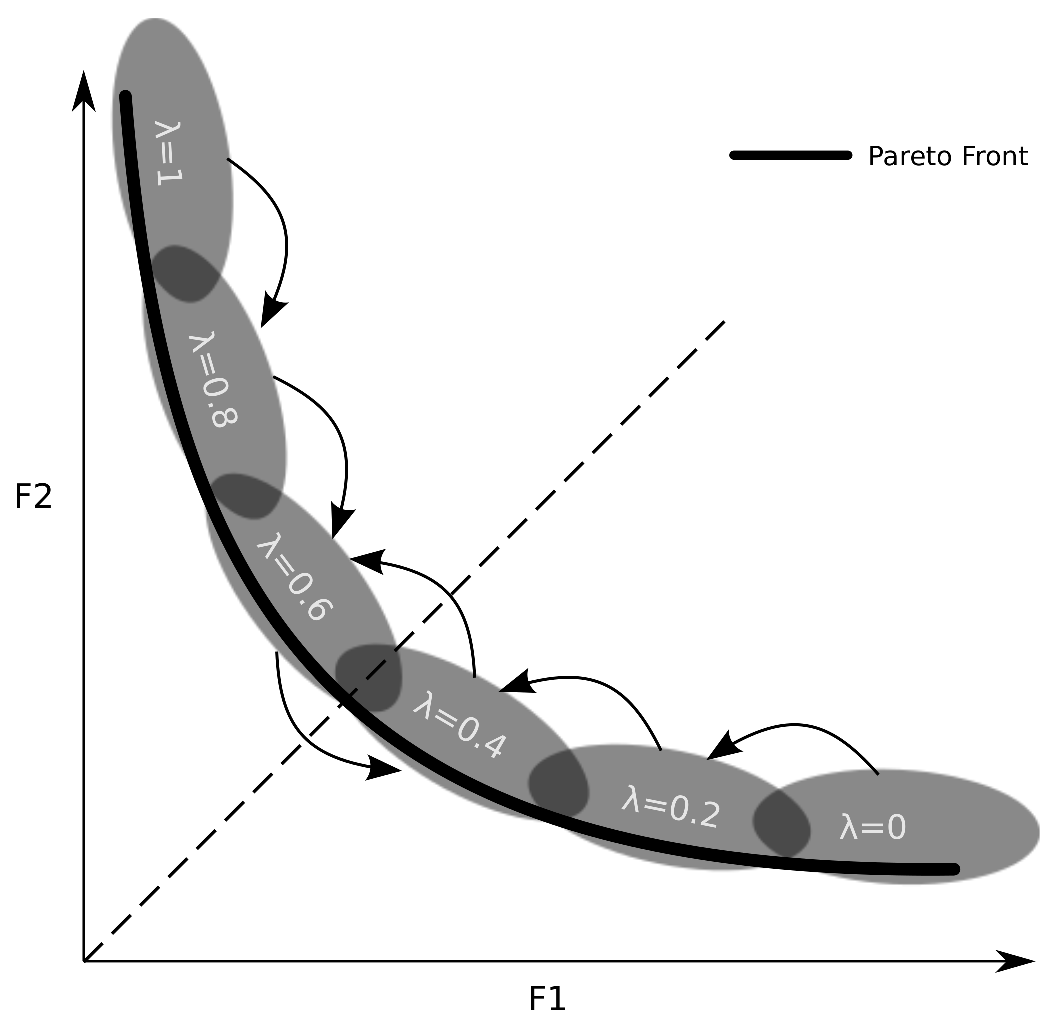
\includegraphics[scale=0.35]{figures/pareto-island-lambda-unidir.eps}}
%\subfigure[Bidirectional topology scheme]{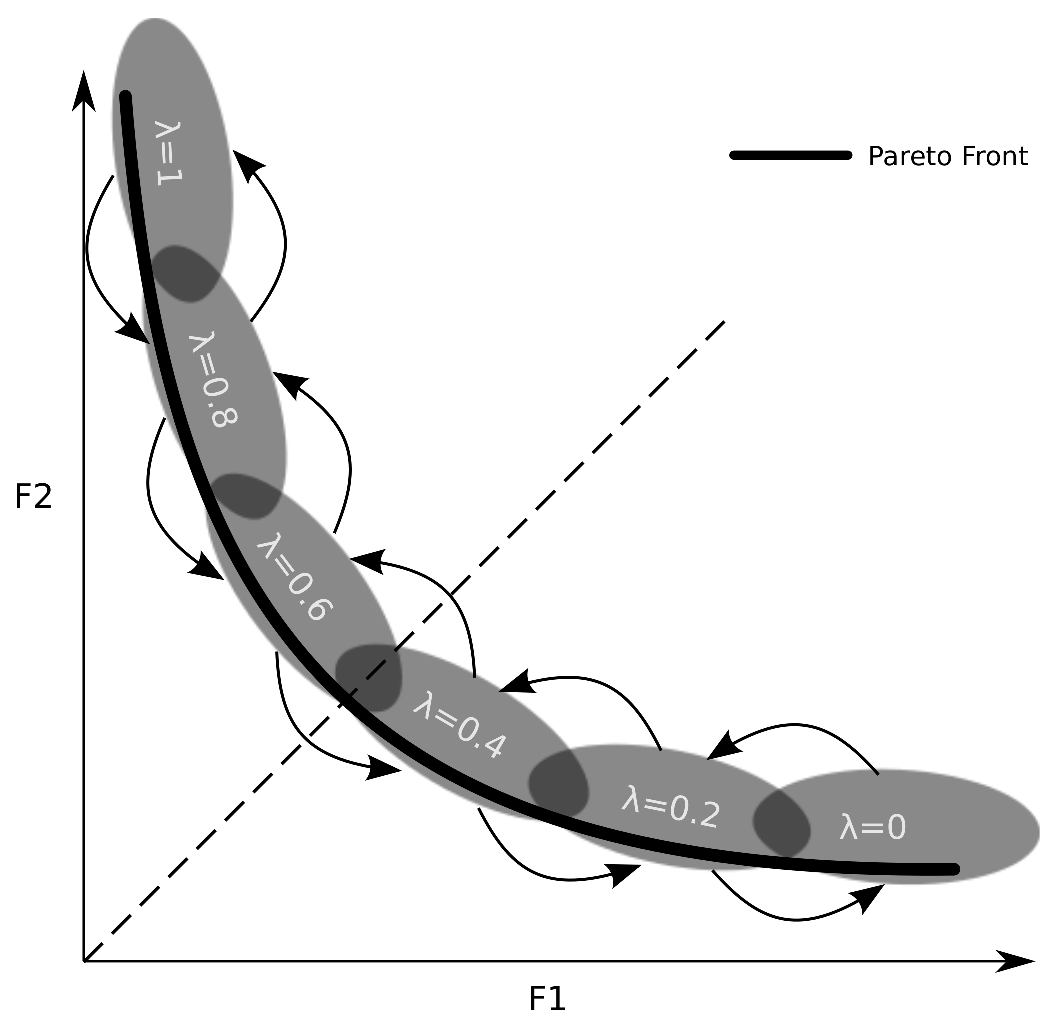
\includegraphics[scale=0.35]{figures/pareto-island-lambda-bidir.eps}}
%\subfigure[Broadcast topology scheme]{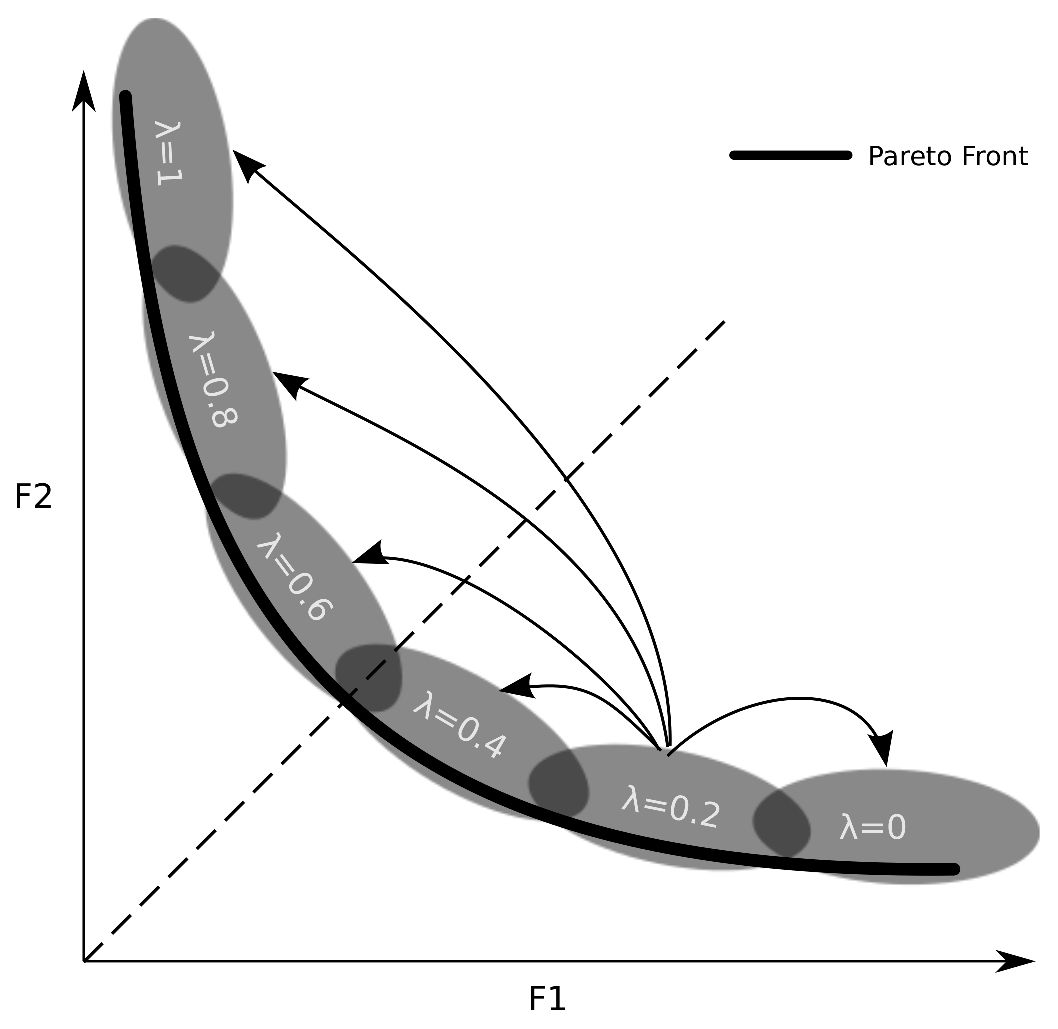
\includegraphics[scale=0.35]{figures/pareto-island-lambda-broadcast.eps}}
%\caption{Pareto-based island model schemes examples for six islands. Each neighborhood migration topology aims to explore the whole Pareto front. The arrows show the migration flows between islands, in order to cover the gaps between colonies/islands. For the sake of clarity broadcast scheme just presents the migrations from one of the islands (to the others), but the model migrates individuals from every island to the rest. The dashed line represents the value $\lambda=0.5$. 
%\label{fig:pareto_island_topologies}}
%\end{center}
%\end{figure}
%
%
%
\begin{figure}[htp!]
\begin{center}
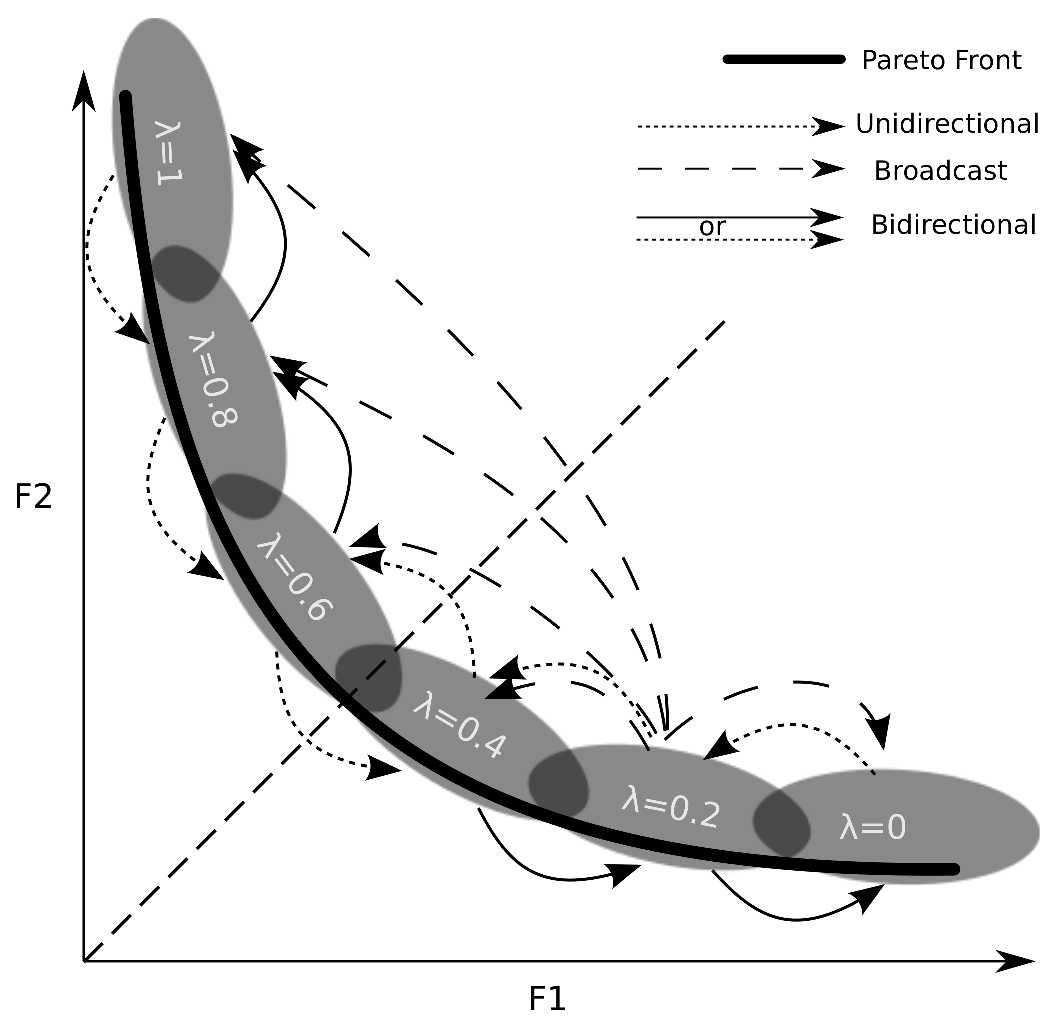
\includegraphics[scale=0.35]{figures/todojunto.eps}
\caption{Pareto-based island model schemes examples for six islands. Each neighborhood migration topology aims to explore the whole Pareto front. The arrows show the migration flows between islands, in order to cover the gaps between colonies/islands. For the sake of clarity broadcast scheme just presents the migrations from one of the islands (to the others), but the model migrates individuals from every island to the rest. The dashed line represents the value $\lambda=0.5$. 
\label{fig:pareto_island_topologies}}
\end{center}
\end{figure}



%---------------------------------
%\subsection{Model justification}
%---------------------------------
%
%As stated in Section \ref{sec:stateofart}, very few researches has been devoted to propose or study island-based models for ant colony optimization algorithms, following any of the common communication/migration topologies \cite{ParallelACO_Island_Topologies}, such as: ring, fully connected, small-world or random. But those studies have been focused on ACOs for solving mono-objective problems.
%
%There are also some works which present multi-colony approaches with communication between the colonies, but they are different to this proposal.
%Iredi's \textit{Bicriterion MC} \cite{BiANT-Iredi} for instance, present a model where the ants update the pheromone matrix of the colonies placed in the PF area where the solution has been found, regardless in which sub-colony they are included. The aim was to increase the exploring area of the colonies, but it presented the problem that the central zone of the obtained PS is much more populated of non-dominated solutions than the bounds (as proved the work \cite{MOACOs_taxonomy}).
%
%In the proposed \textit{Pareto-based island model} (termed just island model from now on) the update is performed in all the pheromone matrixes (per island) so, in principle, all the areas are equally explored, even the bounds. Moreover the novel Pareto-based neighborhood topology has as aim covering the inter-colonies (islands) gaps which could be the main problem of the sub-colony approach, aiding the ants in every colony to explore in other (but close) areas of the PF. 
%
%Other example is described by Kr�ger et al. \cite{Multi-colony_pheromone} where the pheromone matrixes are migrated instead of just the best solutions as in the proposed method, but which is much more expensive in computational time.


%%%%%%%%%%%%%%%%%%%%%%%%%%%%%%%   EXPERIMENTS  %%%%%%%%%%%%%%%%%%%%%%%%%%%%%%%%
%
\section{Experiments and results}
\label{sec:experiments}
%

In order to test the proposed model, with the different neighborhood migration topologies and migration rates, several experiments have been conducted using three different instances of the symmetric TSP\footnote{Available from \url{http://comopt.ifi.uni-heidelberg.de/software/TSPLIB95/}}, in sizes 100, 150 and 200 cities. $kroA$ and $kroB$ instances have been taken in every case, considering each of them as one independent objective of a bi-criteria TSP (bTSP). These problems, named respectively \textit{kroAB100}, \textit{kroAB150} and \textit{kroAB200}, have been widely used in the literature. %\cite{MOACOs_taxonomy,MOACOs_parameters,MOACO_decomposition_bTSP}.
In this case, due to the huge amount of data and figures generated, and considering the space limitations, we will analyze just the results for the hardest one, kroAB200, being the others equivalent, so the conclusions reached for this instance can be extended to the others.

The twelve approaches (MOACS, topology + migration rate) have been run in a cluster platform using 16 processors, being each of them a 2.6 GHz AMD Opteron (AMD64e) with 2GB of memory running Linux.
The cluster has a shared-memory architecture which allows running large threaded jobs (e.g. OpenMP) as well as message-passing jobs. 
The parallelization has been implemented using the Message Passing Interface (MPI), not using the shared memory but the own memory of every processor.

Table \ref{tab:moacs-params} shows the parameter setting for MOACS algorithm and the variations in neighborhood topology and migration rate.
They have been set starting from standard values and performing a systematic experimentation process for fine-tuning them. 

\begin{table}[ht]
\centering
\caption{Parameter values used in MOACS algorithm (in every island).
\label{tab:moacs-params} }
{\small
\begin{tabular}{|l|c|}
\hline
\textit{Num. iterations} & 1000 \\
\textit{Num. ants} & 4 per island \\
%\textit{$\alpha$} (pheromone weight) & 1 \\
\textit{$\beta$} (heuristic weight) & 2 \\
\textit{$q_0$} (pseudo-proportional factor) & 0.8 \\
\textit{$\rho$} (global evaporation rate) & 0.2 \\
\textit{$\varphi$} (local evaporation rate) & 0.1 \\
\hline
\textit{Num. iterations in Local Search (2-OPT)} & 15 \\
\hline
& unidirectional \\
\textit{Migration topology} & bidirectional \\
& broadcast \\
\hline
\textit{Migration rate} & 25, 50, 75, 100 \\

\hline
\end{tabular}
}
\end{table}

The number of iterations and ants per island are the same considered in the previous work. It should be noticed that the value for $q_0$ is smaller than
usual in ACSs (normally very close to 1), in order to choose in the STR paths which are not the most promising (in principle) more than usual. Moreover, the
global evaporation rate ($\rho$) takes a value doubled considering most works, in order to get a faster evaporation of the ant's trails. The reason in both cases is the aim of having a higher exploration component. 
%*** ACLARAR MEJOR ESTO ***

The first study makes a comparison between the different PSs obtained by each configuration. To this end the \textit{median attainment surfaces}\cite{Attainment_Funcs} have been obtained for every approach, considering the solutions of 20 runs (PSs) for every approach.
Each attainment surface graphically shows the distribution of the solutions, summarizing in a graph the outcomes of several runs, by dividing the space of solutions in two parts: the attained solutions (in a percentage) and those not attained. A median attainment surface plots the graph which limits a region in the space attained by the 50\% of the runs.
We have used the software implemented by Knowles\footnote{Available from: \url{http://dbkgroup.org/knowles/plot_attainments/}} considering resolution 100.

The graphs\footnote{Better quality graphs can be found at: \url{ http://my\_url/papers/i-moacos\_gecco}} for each neighborhood migration topology, using every migration rate are plotted in Figure \ref{fig:att_func_topologies}.
%
\begin{figure*}[htp]
\begin{center}
\subfigure[Unidirectional topology]{\includegraphics[scale=0.2,angle=-90]{figures/attainment_unidirectional.eps}}
\subfigure[Bidirectional topology]{\includegraphics[scale=0.2,angle=-90]{figures/attainment_bidirectional.eps}}
\subfigure[Broadcast topology]{\includegraphics[scale=0.2,angle=-90]{figures/attainment_broadcast.eps}}
\caption{Attainment Surfaces of each topology approach for MOACS in kroAB200 problem. Each graph shows the results for every migration rate.
\label{fig:att_func_topologies}}
\end{center}
\end{figure*}
%
In it, it can be seen that all the attainment functions are similar (very close). Thus we cannot extract relevant conclusions from these graphs so, in principle, almost all the migration rates could be a good option. Maybe it could be considered as the best those yielded for the migration rate 100 in every migration topology model (as we will probe in the metrics results). 
Having this in mind, a comparison between the best attainment function graphs is shown in Figure \ref{fig:att_func_best}.
%
\begin{figure}[htp]
\begin{center}
\includegraphics[scale=0.3,angle=-90]{figures/attainment_best.eps}
\caption{Attainment Surfaces of the best results on each topology approach for MOACS in kroAB200 problem.}\label{fig:att_func_best}
\end{center}
\end{figure}

Looking at this figure, we can conclude that \textit{broadcast} model is the worse in this sense, due to the higher exploration factor which means a lower exploitation component than the others, and thus, worse quality in the set of solutions.
In the comparison between \textit{unidirectional} and \textit{bidirectional}, the latter performs better in some specific areas (mainly in the gaps between islands), but the first obtains a wider set of solutions in the bounds and better quality ones in the center of the island's search areas (it has a higher exploitation component).

In order to do a fair comparison, some multi-objective metrics and indicators have been computed for every approach, considering diversity, distribution, convergence and general quality. They are:

\begin{itemize}
    \item \textit{Hypervolume} ($HV \in [0,1]$): it calculates the volume, in the objective space, covered by a set of non-dominated solutions (PS). A higher value means a better result, being 1 the maximum.
    \item \textit{Spread} ($Spr \in [0,1]$): it measures the extent of spread of a set of non-dominated solutions. It considers the Euclidean distance between consecutive solutions on average and extreme distances. A value 0 means an ideal spread.
    \item \textit{Epsilon indicator} ($\epsilon$): it is a measure of the smallest distance it would be necessary to translate every solution in a PS so that it dominates the optimal PF of the problem. Smaller values are better.
    \item \textit{Cardinality of the Pareto set} ($|PS|$): number of non-dominated solutions in the obtained PS.
\end{itemize}

We have used $jMetal$ software \cite{jMetal_CEC10} \footnote{Available from \url{http://jmetal.sourceforge.net/}} to compute them. As a clarification point, a pseudo-optimal Pareto set has been created per each problem, since some of the applied metrics and indicators require an optimal Pareto set to be computed. This, named $PS_G$, has been built by combining all the solutions yielded by all the approaches in the 20 runs; then the dominated solutions have been removed. 

The results are presented in the boxplots in Figure \ref{fig:box_metrics}.
%
\begin{figure}[htp]
\begin{center}
\subfigure[$HV$]{\includegraphics[scale=0.17]{figures/boxplot_hypervolume_gray.eps}}
\subfigure[$Spr$]{\includegraphics[scale=0.17]{figures/boxplot_spread_gray.eps}}
\subfigure[$\epsilon$]{\includegraphics[scale=0.17]{figures/boxplot_epsilon_gray.eps}}
\subfigure[$|PS|$]{\includegraphics[scale=0.17]{figures/boxplot_num_solutions_gray.eps}}
%\subfigure[$Time$]{\includegraphics[scale=0.17]{figures/boxplot_time_gray.eps}}
\caption{Boxplots showing the metrics and indicators values of the 20 PSs (one per run) for the kroAB200 instance of the problem. The topology models are plotted in different shades of gray. Each one of the approaches (topology + migration rate) is labelled with its two initial letters and the migration rate value, from unidirectional-25 to broadcast-100.
\label{fig:box_metrics}}
\end{center}
\end{figure}
%
%\begin{figure}[ht]
%\begin{center}
%\includegraphics[scale=0.17]{figures/boxplot_hypervolume_gray.eps}
%\caption{Boxplots showing the $hypervolume\; metric\; (HV)$ values of the 20 PSs (one per run) for the kroAB200 instance of the problem. The topology models are plotted in different shades of gray. Each one of the approaches (topology + migration rate) is labelled with its two initial letters and the migration rate value, from unidirectional-25 to broadcast-100.
%\label{fig:box_hypervolumes}}
%\end{center}
%\end{figure}
%
The $HV$ results in Figure \ref{fig:box_metrics}.(a) show that \textit{unidirectional} solutions have better quality than the solutions obtained by the other topologies, due to its higher exploitation component which means more optimal solutions are yielded. \textit{Bidirectional} results are similar but worse, because it has a higher exploration factor, and \textit{broadcast} has obtained the worst, since it is the most explorative method. With respect to the \textit{migration rates}, 100 seems to yield the best results. It is not surprising considering that a higher migration rate means less migration events are performed and thus, less ants migrate and influence in the search of the other islands, i.e., the exploration factor is decreased. So the higher the migration rate is, the higher the exploitation component is in every island, and the better the solutions are achieved.

%\begin{figure}[htp]
%\begin{center}
%\includegraphics[scale=0.17]{figures/boxplot_spread_gray.eps}
%\caption{Boxplots showing the $spread\; indicator\; (Spr)$ values of the 20 PSs (one per run) for the kroAB200 instance of the problem. The colors and labels are the same as in previous figure.
%The topology models are plotted in different shades of gray. Each one of the approaches (topology + migration rate) is labelled with its two initial letters and the migration rate value, from unidirectional-25 to broadcast-100.
%\label{fig:box_spread}}
%\end{center}
%\end{figure}
%
Figure \ref{fig:box_metrics}.(b) shows this time the contrary situation, being \textit{broadcast} the best option with regard to the spread/distribution ($Spr$) of solutions, i.e. to the wide of the Pareto set. The reason is the same as before but on the contrary sense. Thus the higher the exploration component is, the wider the PS is.
As expected, the lowest value for the \textit{migration rate} yields the best results for this indicator (closer to 0).

%\begin{figure}[htp]
%\begin{center}
%\includegraphics[scale=0.17]{figures/boxplot_epsilon_gray.eps}
%\caption{Boxplots showing the $epsilon\; metric\; (\epsilon)$ values of the 20 PSs (one per run) for the kroAB200 instance of the problem. 
%The colors and labels are the same as in previous figure.
%The topology models are plotted in different shades of gray. Each one of the approaches (topology + migration rate) is labelled with its two initial letters and the migration rate value, from unidirectional-25 to broadcast-100.
%\label{fig:box_epsilon}}
%\end{center}
%\end{figure}
%
$\epsilon$ metric results (in Figure \ref{fig:box_metrics}.(c)) show that the best convergence factor is reached by the \textit{bidirectional} approach, and for high values of the \textit{migration rates} (75 and 100). The reason lies in the higher exploitation performed in this model in every island, since the migrants are solutions from close search areas. High values of the \textit{migration rate} lead to less migration events, so the algorithm can perform more iterations to improve the solutions in an area, i.e. the exploitation grows and the obtained solutions are closer to the optimal ones.

%\begin{figure}[htp]
%\begin{center}
%\includegraphics[scale=0.17]{figures/boxplot_num_solutions_gray.eps}
%\caption{Boxplots showing the number of solutions (cardinality, $|PS|$) of the 20 PSs (one per run) for the kroAB200 instance of the problem. 
%The colors and labels are the same as in previous figure.
%The topology models are plotted in different shades of gray. Each one of the approaches (topology + migration rate) is labelled with its two initial letters and the migration rate value, from unidirectional-25 to broadcast-100.
%\label{fig:box_num_sols}}
%\end{center}
%\end{figure}
%
With respect to $|PS|$ (cardinality), plotted in Figure \ref{fig:box_metrics}.(d), high values for \textit{migration rate} correspond to higher number of solutions in the PS. \textit{unidirectional} model seems to show the best performance in this sense. Thus, the exploitation is more desirable in this problem, because more non-dominated solutions are obtained in the specific search area of every island, than close to the neighbors (when more migrants arrive to an island).

The final boxplot (Figure \ref{fig:box_time}) considers the distributed nature of the model, and shows the running time results. The worst time among all the processors in one execution has been chosen as the running time of that execution.

\begin{figure}[htp]
\begin{center}
\includegraphics[scale=0.17]{figures/boxplot_time_gray.eps}
\caption{Boxplots showing the running time (in milliseconds) of the 20 runs for the kroAB200 instance of the problem. 
The colors and labels are the same as in previous figure.
%The topology models are plotted in different shades of gray. Each one of the approaches (topology + migration rate) is labelled with its two initial letters and the migration rate value, from unidirectional-25 to broadcast-100.
\label{fig:box_time}}
\end{center}
\end{figure}
%
Looking at this figure, it can be noticed that \textit{bidirectional} model consumes the highest computational time. These results may seem not expected, since, in principle, there should be more communication costs in the broadcast model. The main reason lies in the algorithm implementation, since the PS updating is quite expensive. Thus in \textit{bidirectional} model there are several updates due to found solutions in the inter-colony gaps, because of the exploitation factor increasing that the migrations in this model provide (close solutions in the same area are received). This along with a higher communication cost than \textit{unidirectional} model leads to these results. In the \textit{broadcast} case, the communication costs are higher, but there are many fewer updates in the PS, since it finds less non-dominated solutions than the other models. This conclusion is supported by the similar results obtained for the different \textit{migration rates}, which should increase the running time consumption when these rates decrease, however it does not happen. Thus communication cost is not the main factor in these results.
Anyway the differences are around 3 seconds, so they are not significative from the user point of view.

Finally, ANOVA statistical tests \cite{ANOVA_Fisher} have been applied to complete this analysis. These tests allow us to determine whether a change in the results of every metric is due to a change in a factor or to a random effect. In this case, the factors to consider are the possible approaches (topology + migration rate). 
After applying ANOVA, if the test has shown significative differences, post-hoc Tukey's Honestly Significant Difference (HSD) test \cite{Tukey_HSD} has been applied to find which factors are causing these differences. 

The ANOVA results are shown in Table \ref{tab:anova}. It can be noticed that the approaches (topologies + migration rates) have significative influence on the values of every metric or indicator, since the \textit{P-value (Sig. Level)} is always much smaller than 0.05 (is the standard minimum value 2.2e-16). Moreover, they have significative influence at a confidence level of $99\%$.
However in the case of $Time$ no influence has been found for \textit{migration rate} factor.

\begin{table}[htp]

\caption{ANOVA test results for the metrics and indicators values. Signif. codes:  0 *** 0.001 ** 0.01 * 0.05.
\label{tab:anova}}
\begin{center}

\begin{tabular}{lr}

$HV$ &

\begin{tabular}{|c|c|c|c|}
\hline
\scriptsize{Param.}		&\scriptsize{Df} &  \scriptsize{F}     & \scriptsize{P (Sig. Level)} \\
\hline
\hline
\scriptsize{\textit{topology}}     &\scriptsize{2}  & \scriptsize{327.219} & \textbf{\scriptsize{$<$ 2.20e-16 ***}} \\
\hline
\scriptsize{\textit{mig. rate}}         &\scriptsize{1}  & \scriptsize{272.867} & \textbf{\scriptsize{$<$ 2.20e-16 ***}} \\
\hline
\scriptsize{Residuals} & \multicolumn{3}{l|}{\scriptsize{234 0.0016073 0.00000687}} \\
\hline
\end{tabular} \\

$\epsilon$ &

\begin{tabular}{|c|c|c|c|}
\hline
%\scriptsize{Param.}		&\scriptsize{Df} &  \scriptsize{F}     & \scriptsize{P (Sig. Level)} \\ 
%\hline
\scriptsize{\textit{topology}}     &\scriptsize{$\;$2$\;$}  & \scriptsize{51.1573} & \textbf{\scriptsize{$<$ 2.20e-16 ***}} \\
\hline
\scriptsize{\textit{mig. rate}}         &\scriptsize{1}  & \scriptsize{32.4955} & \textbf{\scriptsize{ 3.58e-08 ***}} \\
\hline
\scriptsize{Residuals} & \multicolumn{3}{l|}{\scriptsize{234 453518905  1938115}} \\
\hline
\end{tabular} \\

$Spr$ &

\begin{tabular}{|c|c|c|c|}
\hline
%\scriptsize{Param.}		&\scriptsize{Df} &  \scriptsize{F}     & \scriptsize{P (Sig. Level)} \\ 
%\hline
\scriptsize{\textit{topology}}     &\scriptsize{$\;$2$\;$}  & \scriptsize{104.750} & \textbf{\scriptsize{$<$ 2.20e-16 ***}} \\
\hline
\scriptsize{\textit{mig. rate}}         &\scriptsize{1}  & \scriptsize{57.4511} & \textbf{\scriptsize{ 8.06e-13 ***}} \\
\hline
\scriptsize{Residuals} & \multicolumn{3}{l|}{\scriptsize{234 0.36810 0.001573}} \\
\hline
\end{tabular} \\

$|PS|$ & 

\begin{tabular}{|c|c|c|c|}
\hline
%\scriptsize{Param.}		&\scriptsize{Df} &  \scriptsize{F}     & \scriptsize{P (Sig. Level)} \\ 
%\hline
\scriptsize{\textit{topology}}     &\scriptsize{$\;$2$\;$}  & \scriptsize{77.3939} & \textbf{\scriptsize{$<$ 2.20e-16 ***}} \\
\hline
\scriptsize{\textit{mig. rate}}         &\scriptsize{1}  & \scriptsize{28.1965} & \textbf{\scriptsize{ 2.54e-07 ***}} \\
\hline
\scriptsize{Residuals} & \multicolumn{3}{l|}{\scriptsize{234  35762   152.8 }} \\
\hline
\end{tabular} \\


$Time$ &

\begin{tabular}{|c|c|c|c|}
\hline
%\scriptsize{Param.}		&\scriptsize{Df} &  \scriptsize{F}     & \scriptsize{P (Sig. Level)} \\ 
%\hline
\scriptsize{\textit{topology}}     &\scriptsize{$\;$2$\;$}  & \scriptsize{873.522} & \textbf{\scriptsize{$<$ 2.20e-16 ***}} \\
\hline
\scriptsize{\textit{mig. rate}}         &\scriptsize{1}  & \scriptsize{0.1675} & \textbf{\scriptsize{ 0.6828 }} \\
\hline
\scriptsize{Residuals} & \multicolumn{3}{l|}{\scriptsize{234  43473869    185786 }} \\
\hline
\end{tabular}

\end{tabular}
\end{center}
\end{table}

Given this conclusion, post-hoc Tukey's HSD test can be used. It is a versatile, easily calculated technique that allows determining exactly where the significant differences are, once ANOVA has found a significant effect.
This test compares pairs of the factor values, i.e. topology on one side, and migration rate on the other, showing a segment (confidence level) for each comparison. 
Additionally, there is a vertical dotted line (distance equals zero) that intersects some segments. Significant differences can be found in those cases where the vertical line does not intersect a segment (those values compared are significantly different).
Tukey's HSD results can be seen in Figure \ref{fig:tukeyHSD}.

\begin{figure}[htp]
\begin{center}
\subfigure[$HV$]{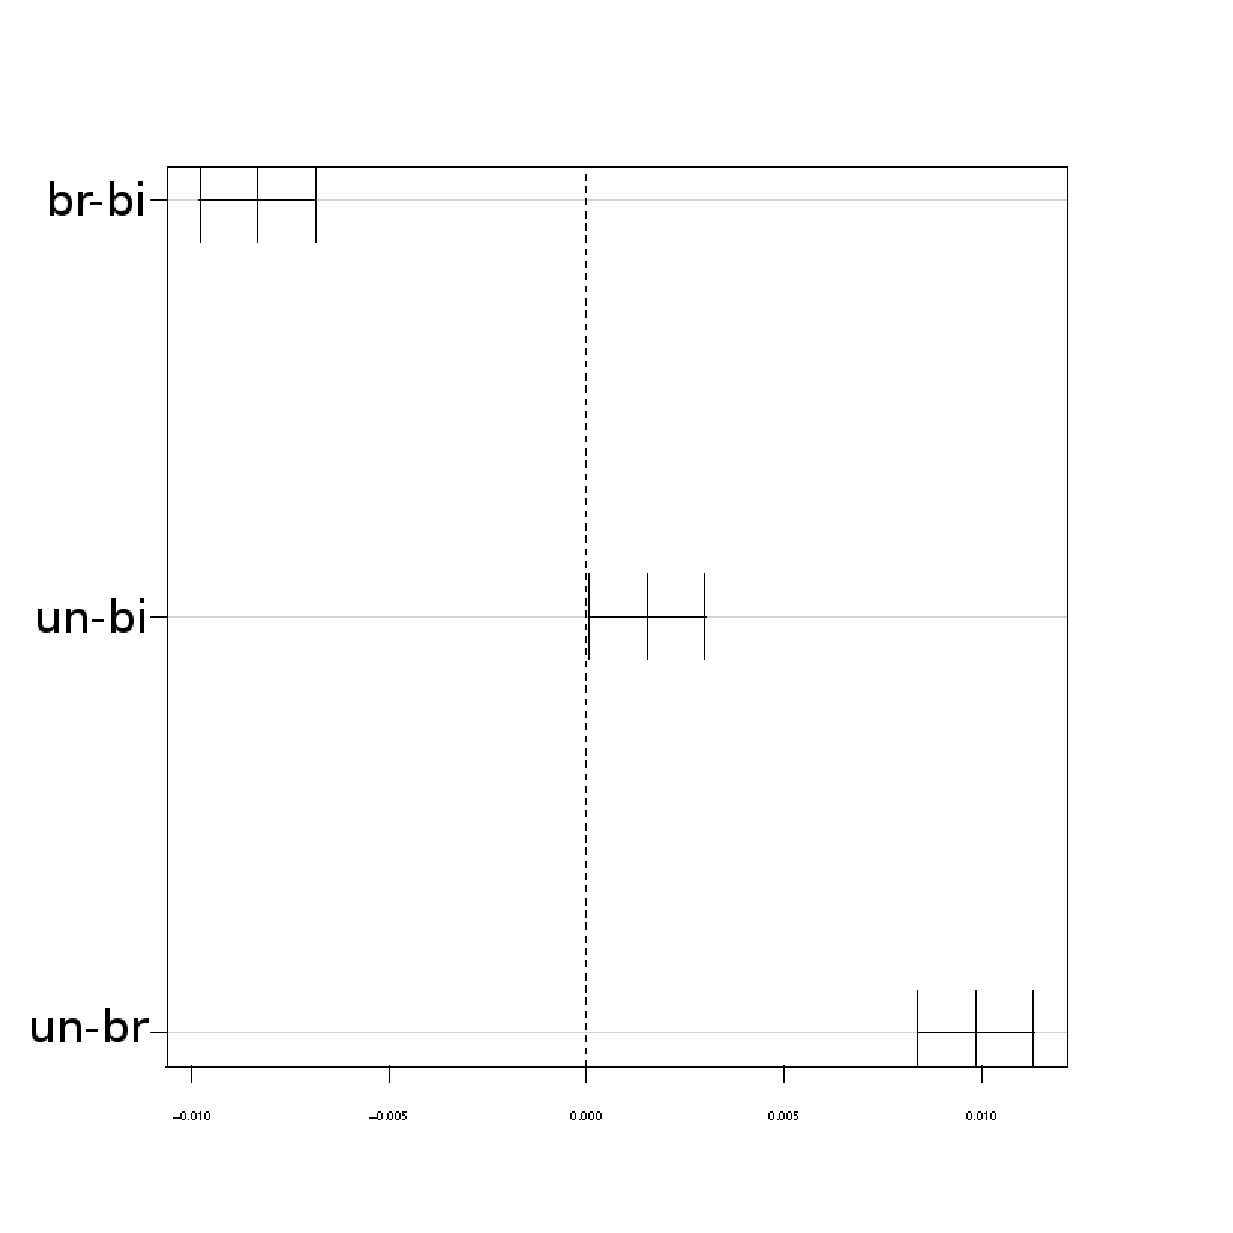
\includegraphics[scale=0.2]{figures/tukey_hypervolume_topology.eps}
		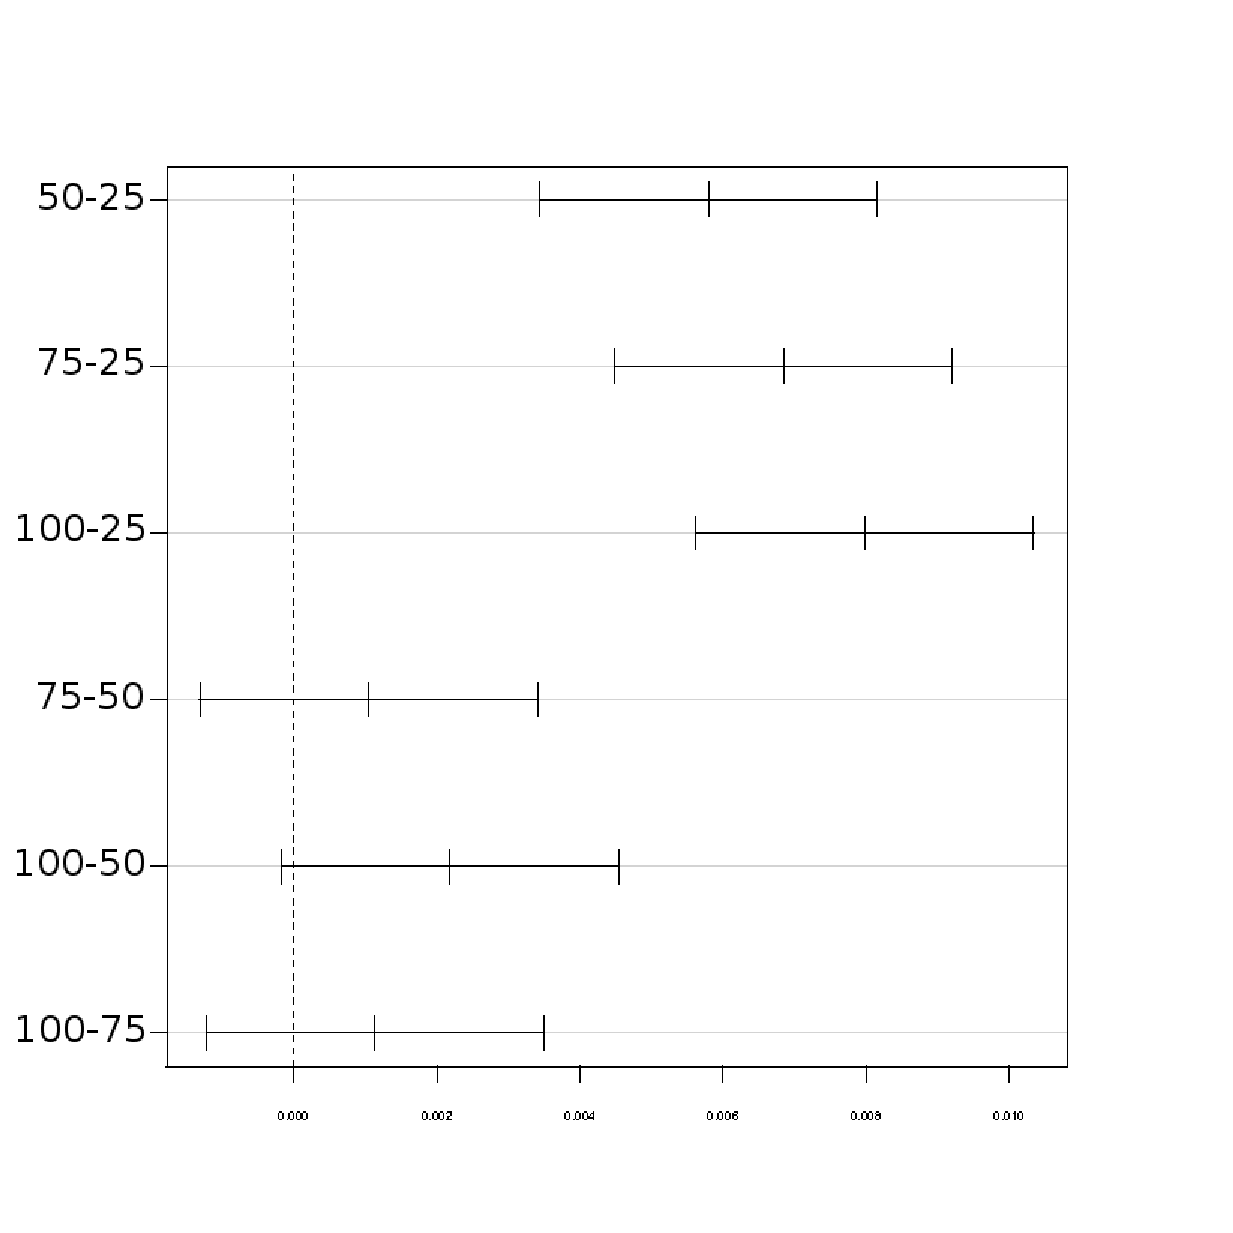
\includegraphics[scale=0.2]{figures/tukey_hypervolume_mig_rate.eps}}
\subfigure[$\epsilon$]{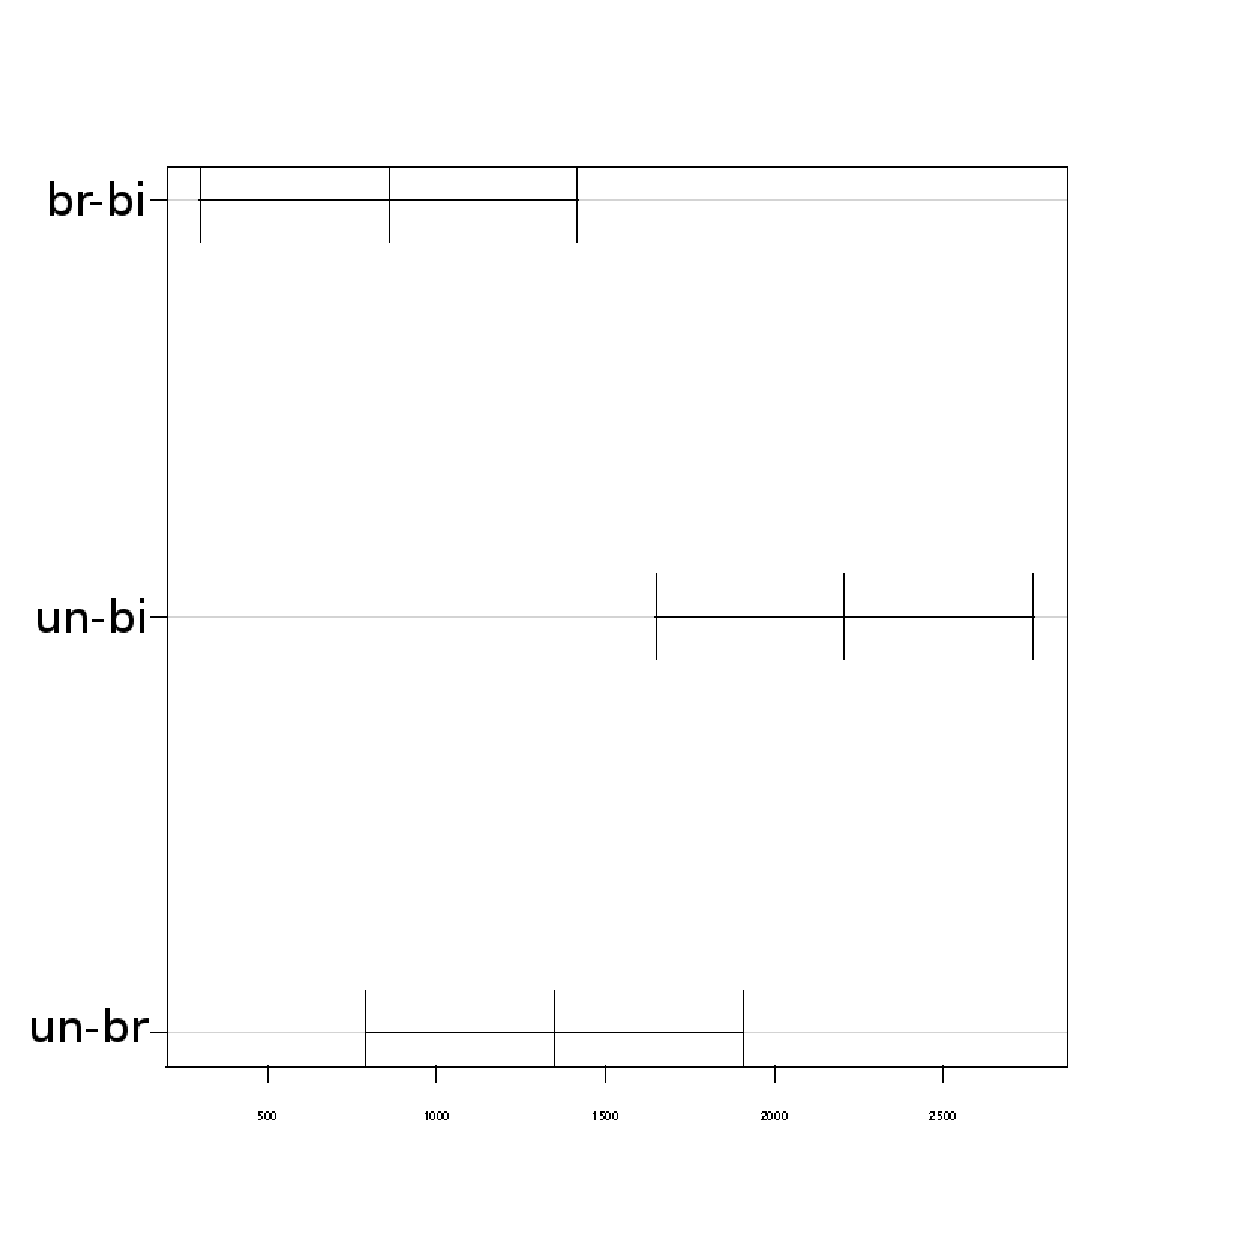
\includegraphics[scale=0.2]{figures/tukey_epsilon_topology.eps}
		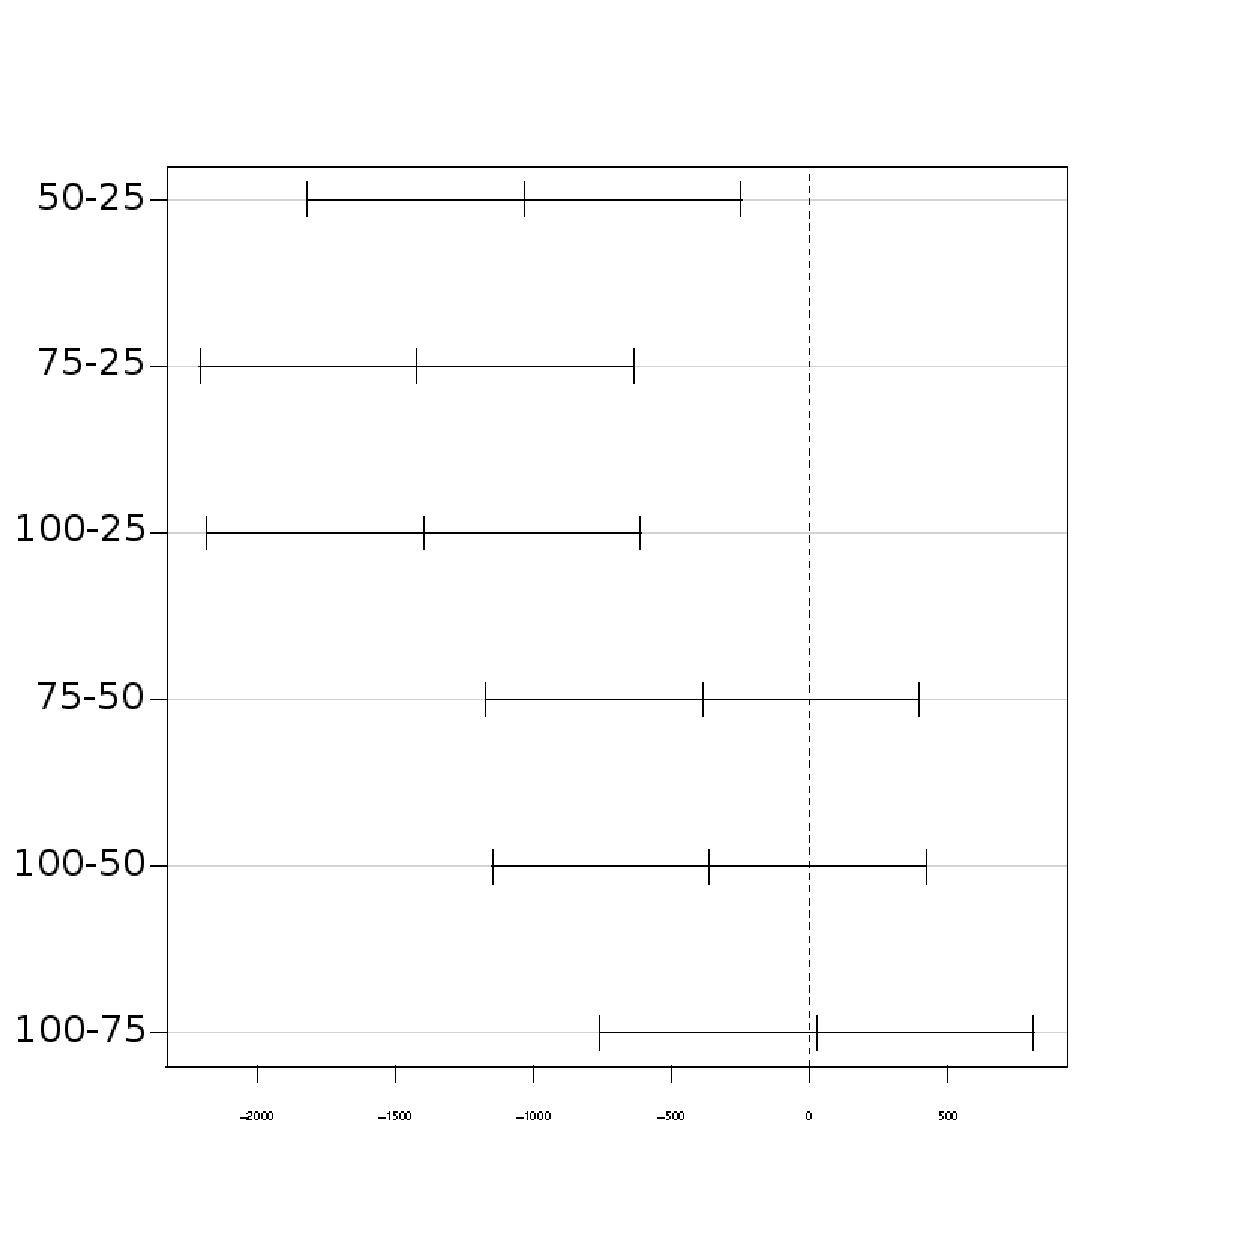
\includegraphics[scale=0.2]{figures/tukey_epsilon_mig_rate.eps}}
\subfigure[$Spr$]{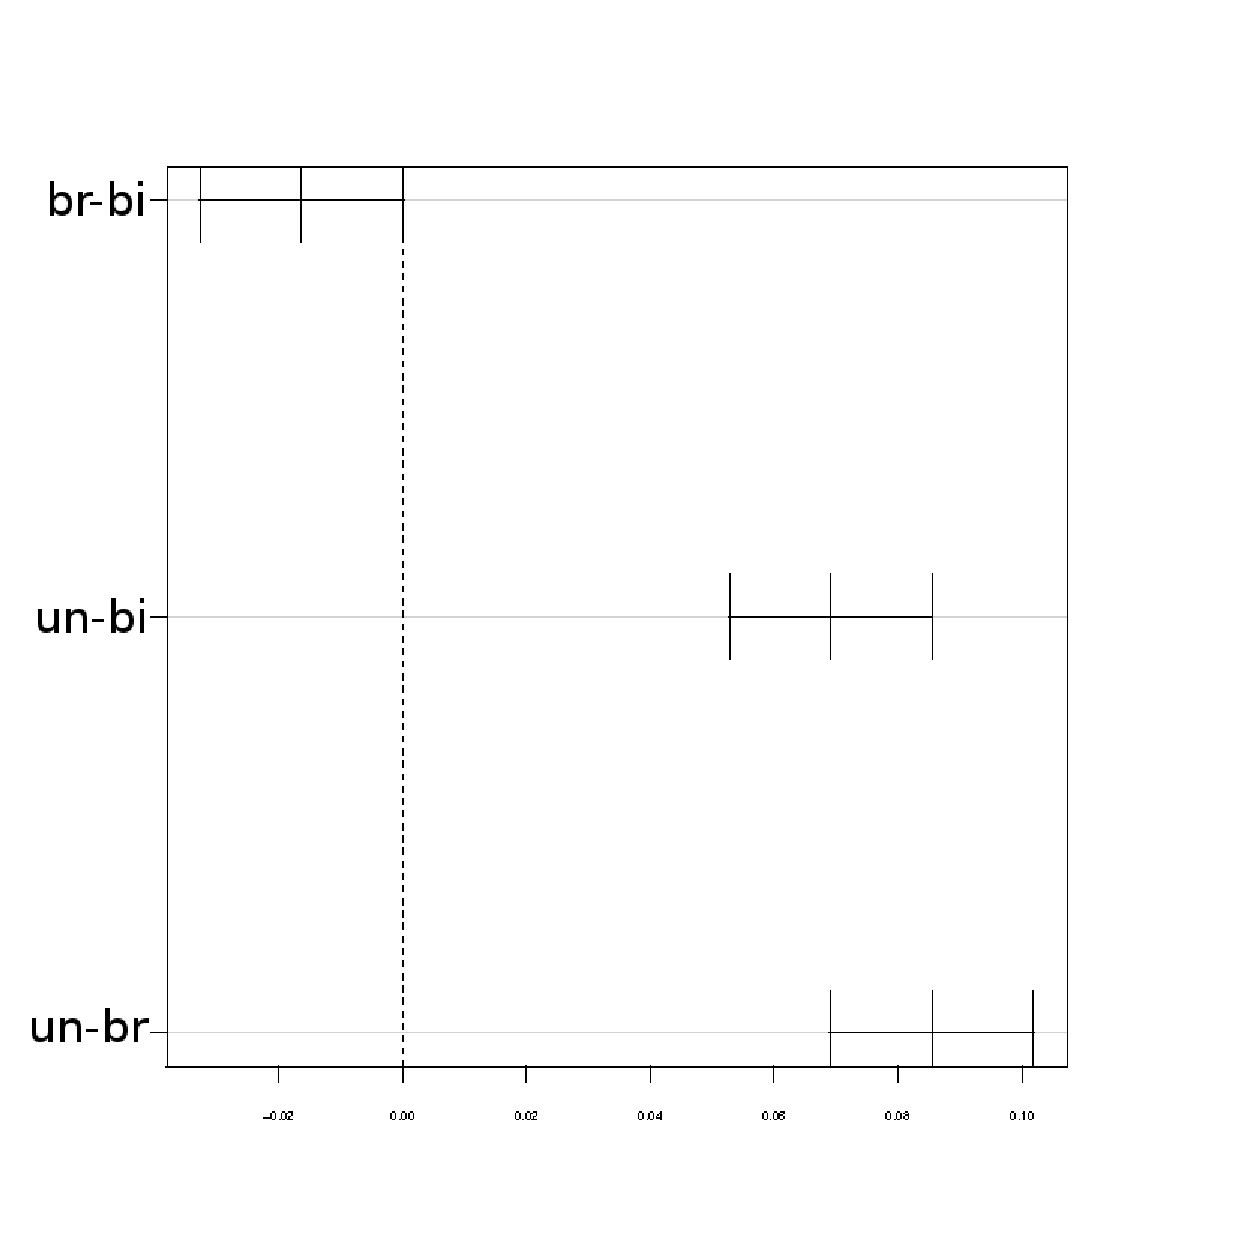
\includegraphics[scale=0.2]{figures/tukey_spread_topology.eps}
		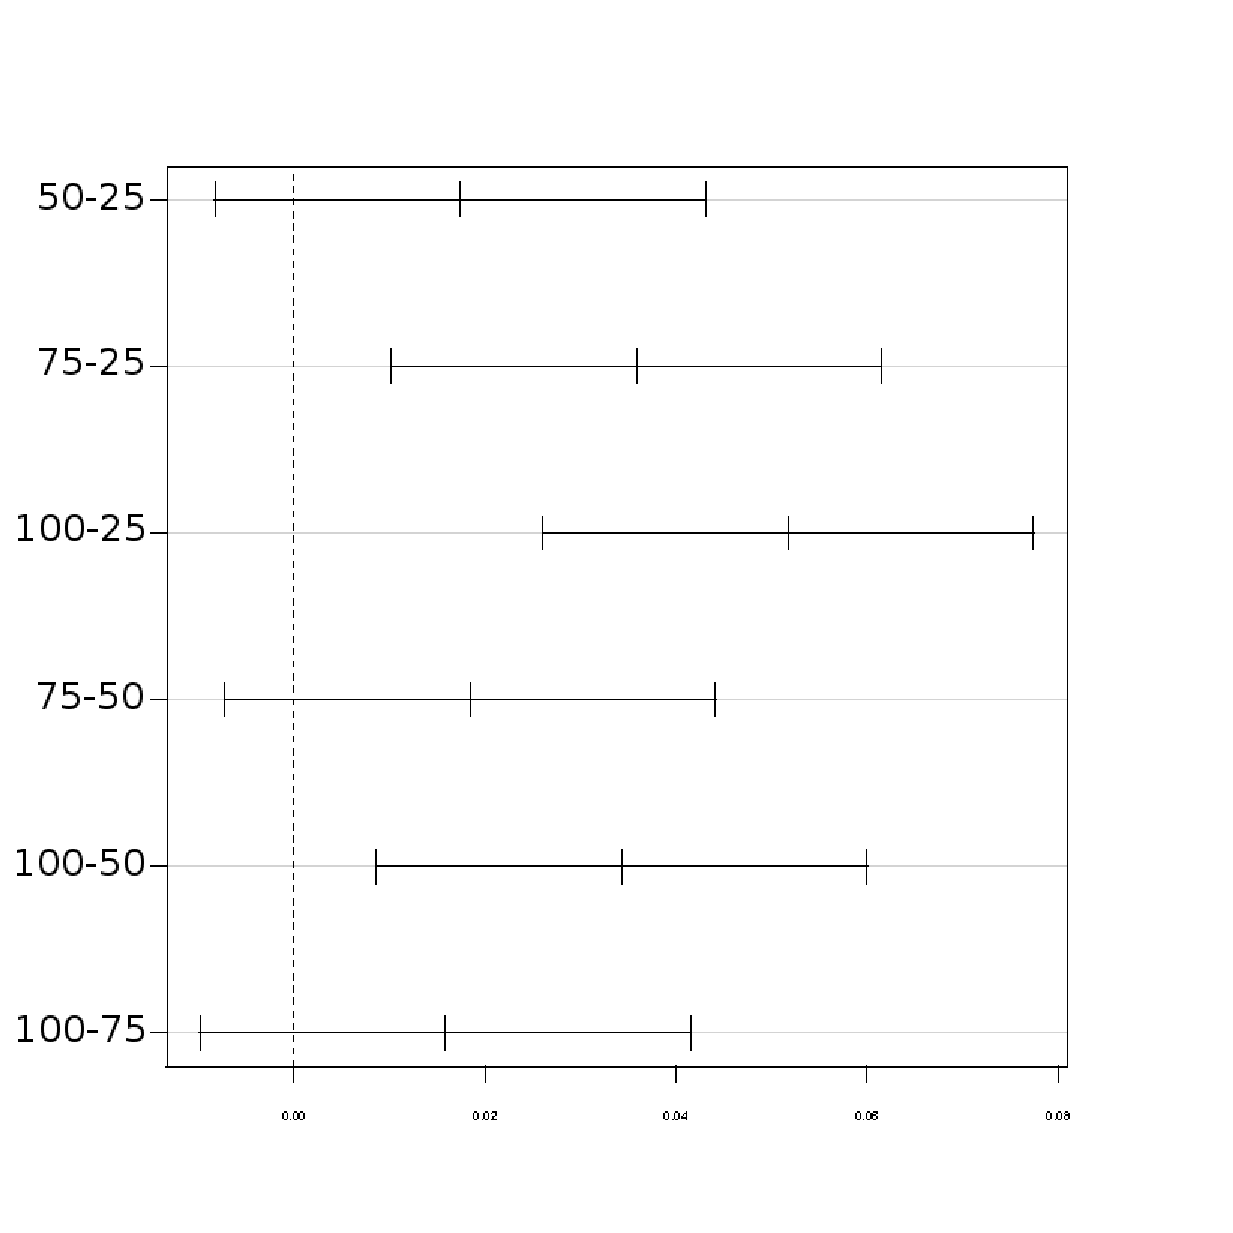
\includegraphics[scale=0.2]{figures/tukey_spread_mig_rate.eps}}
\subfigure[$|PS|$]{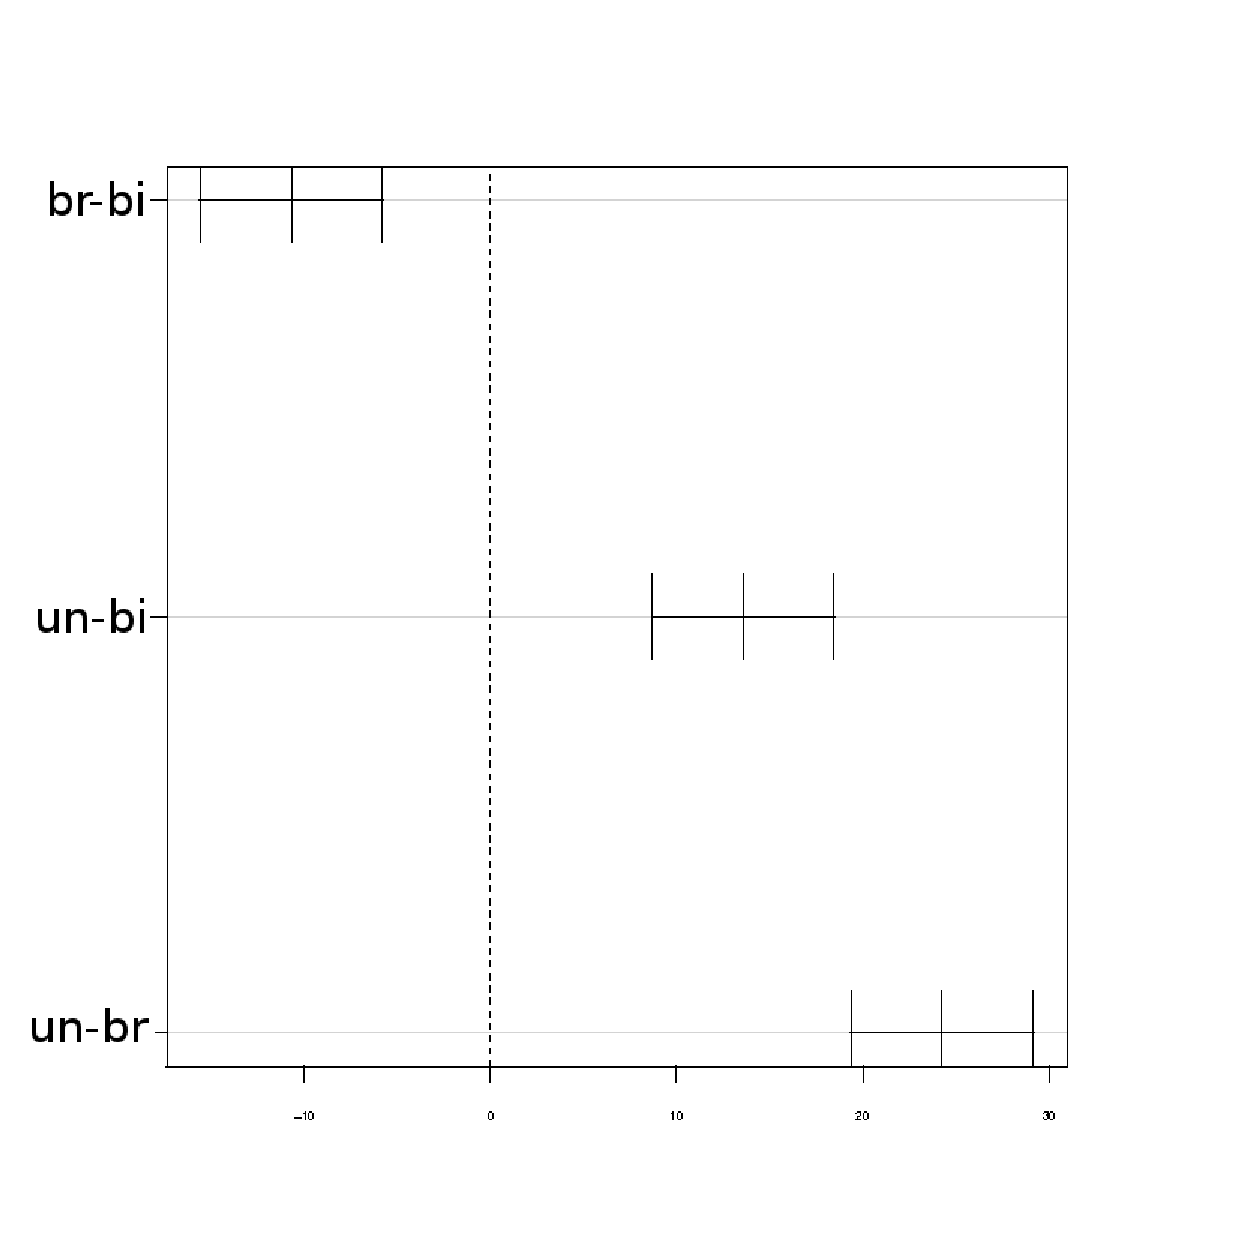
\includegraphics[scale=0.2]{figures/tukey_num_solutions_topology.eps}
		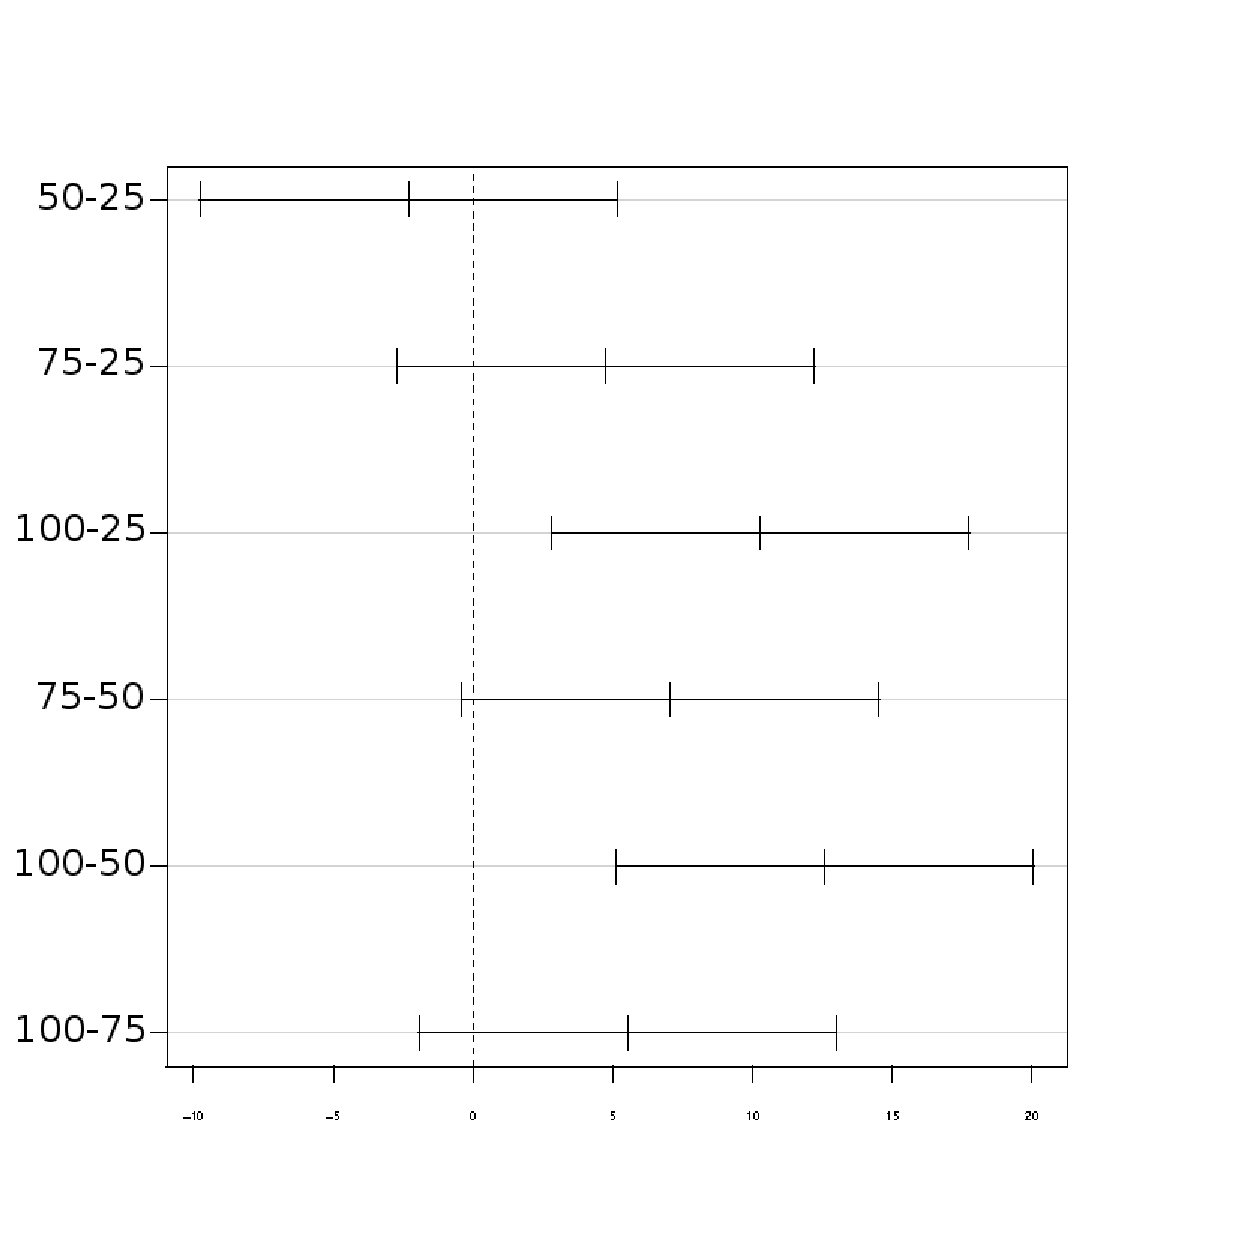
\includegraphics[scale=0.2]{figures/tukey_num_solutions_mig_rate.eps}}
\subfigure[$Time$]{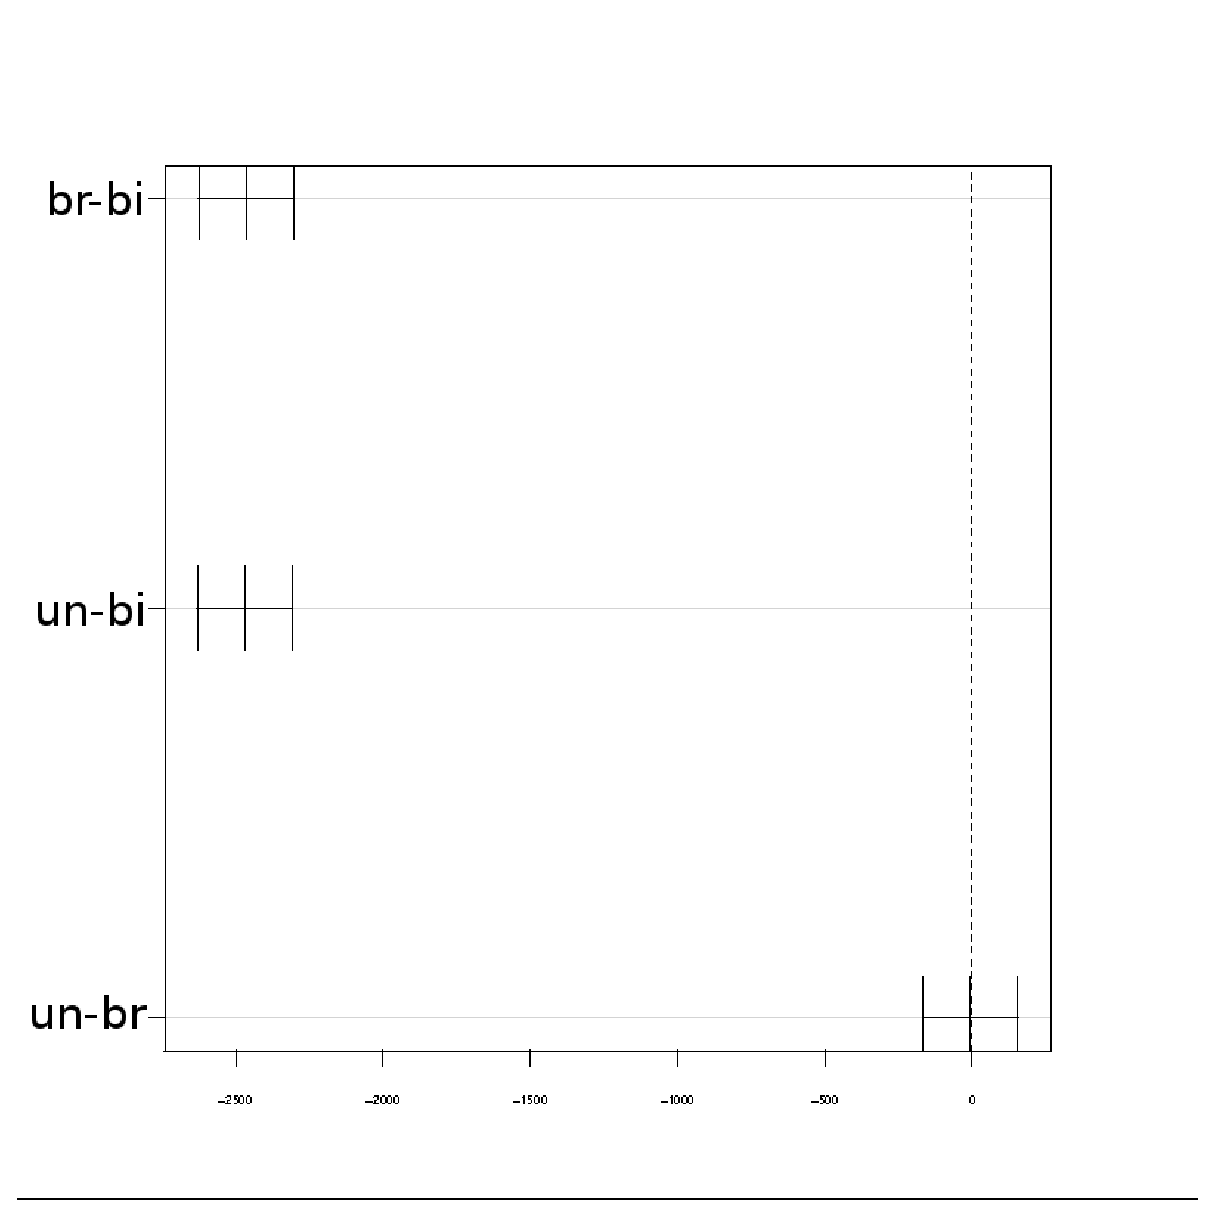
\includegraphics[scale=0.2]{figures/tukey_time_topology.eps}
		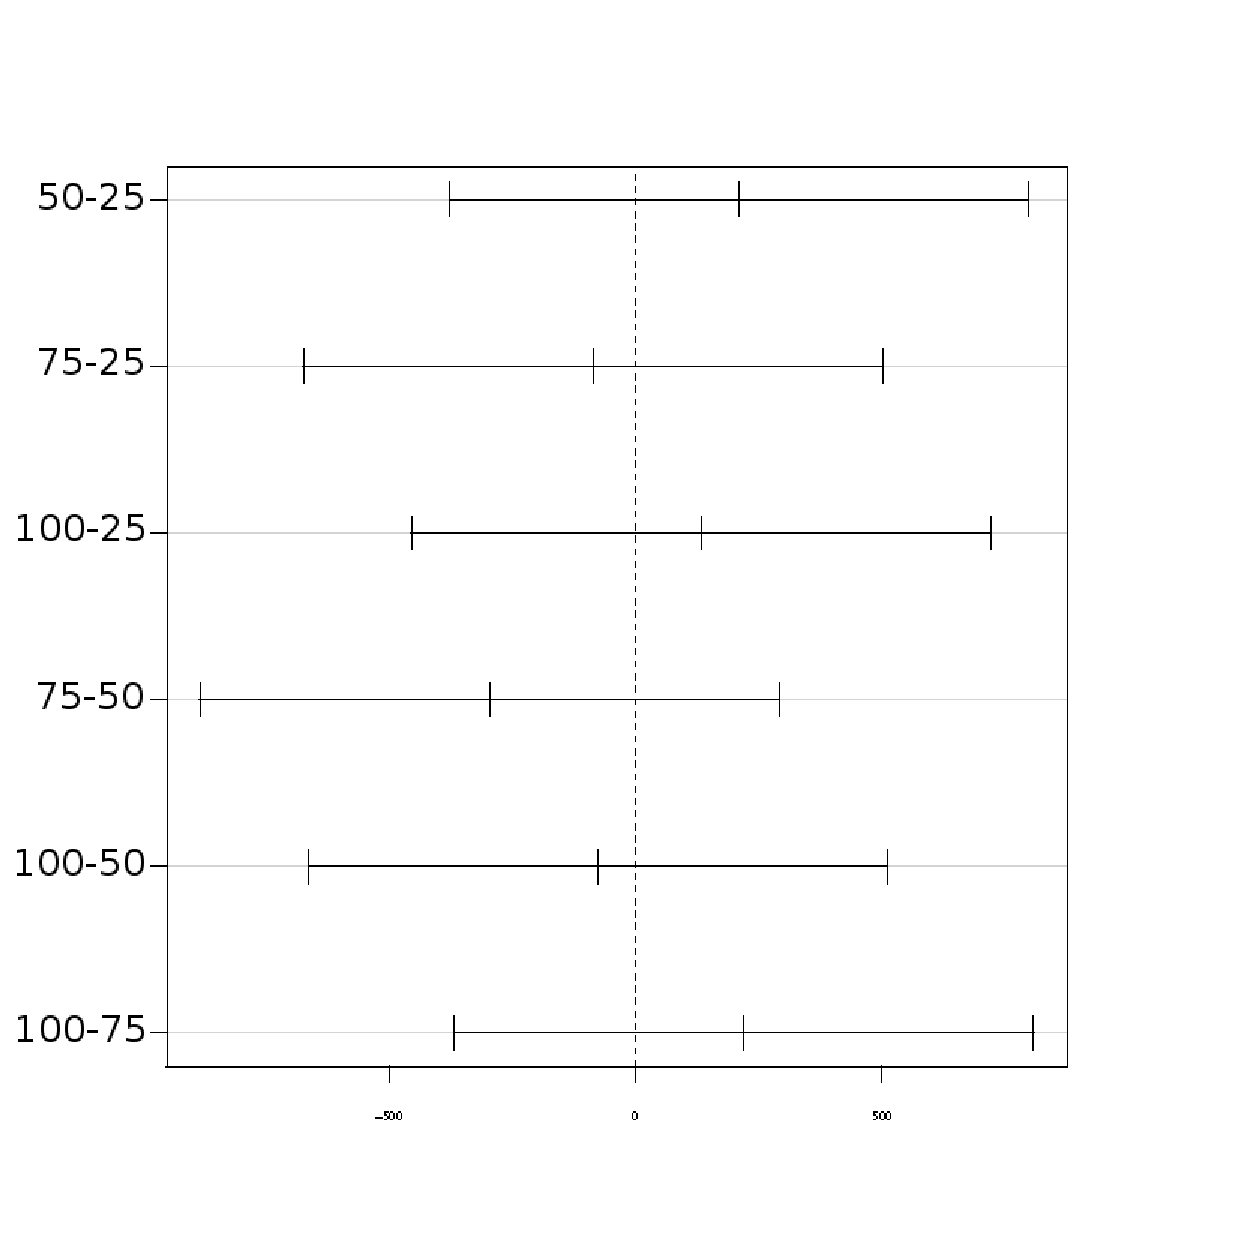
\includegraphics[scale=0.2]{figures/tukey_time_mig_rate.eps}}
\caption{Tukey's HSD graphs for topology (left) and migration rate (right)}\label{fig:tukeyHSD}
\end{center}
\end{figure}
% 
The first conclusion that can be extracted from these graphs is that, in most of cases, there are no significative differences between the results when using close \textit{migration rates}, and just when the difference in rate is more than 50, the differences arise.
With respect the \textit{migration topology}, the differences are always significatives, but in the comparison between \textit{unidirectional} and \textit{bidirectional} in $HV$ metric, between \textit{broadcast} and \textit{bidirectional} in $Spr$ metric, and between \textit{unidirectional} and \textit{broadcast} in $Time$ measure. These facts could be also inferred looking respectively at Figures \ref{fig:box_metrics}.(a), \ref{fig:box_metrics}.(b) and \ref{fig:box_time}.

A set of conclusions can be extracted from the experiments presented in this section:
\begin{itemize}
\item High values for the \textit{migration rate} are recommended for any \textit{migration topology} considered. The balance between the quality of the solutions and their spread obtained for 100 leads us to choose this value as the best.
\item \textit{bidirectional} migration topology can be considered as the best with regard most of the indicators. It gets a good balance between quality, spread and convergence, with the only handicap of requiring higher computational time than the other approaches, and yielding less non-dominated solutions in average, but getting a number close to \textit{unidirectional}.
\item However, if having the smaller running time as possible is considered as a requirement, \textit{unidirectional} turns in the best option when searching for quality in the solutions, and \textit{broadcast} when the aim if get a well distributed PS (good spread).
\end{itemize}


%%%%%%%%%%%%%%%%%%%%%%%%%%%%%%%% CONCLUSIONS %%%%%%%%%%%%%%%%%%%%%%%%%%%%%%%

\section{Conclusions}
\label{sec:conclusions}

This work presents an analysis of the Pareto-based island model introduced in the recent article \cite{iMOACOS_SOCO}. It is a distribution scheme inspired in the island model widely used in evolutionary algorithms. But this is applied in the scope of multi-objective problems and is aimed to distribute a set of sub-colonies in an ant colony optimization algorithm. Thus it is a shape of multi-colony (or coarse-grained) model.

A neighborhood migration topology named \textit{unidirectional} was initially proposed. It is focused on the Pareto front (representation of the ideal set of solutions) shape, so it establish the communication links in order to `cover' the whole Pareto front, i.e. trying that the sub-colonies/islands search in all the possible areas of the space of solutions.
In this paper two additional topologies are presented: \textit{bidirectional}, which completes the communications between islands in both directions, and \textit{broadcast}, which migrates individuals from every island to the rest.

In addition, four different values for the \textit{migration rate} parameter have been tested. The aim is to decide the best combination in these two factors of the proposed island model.
In order to do this, MOACS algorithm \cite{MOACS-Baran} has been implemented using the proposed topologies. It has been adapted to solve the symmetric bi-criteria TSP in three different instances (100, 150 and 200 cities).

Several experiments have been conducted, computing classical metrics and indicators (hypervolume, spread, epsilon), along with graphs (attainment functions). Then a deep analysis of the results has been done in order to determine the approach with the best performance. In addition, statistical tests ANOVA and post-hoc Tukey's HSD have been applied to support this analysis.

The conclusions reached say that high values for the \textit{migration rate} (around 100) yield better results. In the comparison between the \textit{migration topologies}, the \textit{bidirectional} approach has been chosen as the best option due to its good balance between the quality of the obtained solutions and the diversity and convergence level which it gets.

Following this line of work it could be interesting to perform another analysis with regard other factors of the island model, such as the migration or replacement policies. The comparison with others MOACO multi-colony models is another interesting line of research. There are several models proposed in the
literature such as the one by Iredi at al. \cite{BiANT-Iredi}. 
It would be also interesting to conduct a comparison with state-of-the-art multi-objective evolutionary algorithms implementing the island model.

%ACKNOWLEDGMENTS are optional
\section{Acknowledgments}
Thanks to everybody

%
% The following two commands are all you need in the
% initial runs of your .tex file to
% produce the bibliography for the citations in your paper.
\bibliographystyle{abbrv}
\bibliography{imoacos}  % sigproc.bib is the name of the Bibliography in this case
% You must have a proper ".bib" file
%  and remember to run:
% latex bibtex latex latex
% to resolve all references
%
% ACM needs 'a single self-contained file'!
%
%APPENDICES are optional
%\balancecolumns
%\appendix
%Appendix A
%\section{Headings in Appendices}
%The rules about hierarchical headings discussed above for
%the body of the article are different in the appendices.
%In the \textbf{appendix} environment, the command
%\textbf{section} is used to
%indicate the start of each Appendix, with alphabetic order
%designation (i.e. the first is A, the second B, etc.) and
%a title (if you include one).  So, if you need
%hierarchical structure
%\textit{within} an Appendix, start with \textbf{subsection} as the
%highest level. Here is an outline of the body of this
%document in Appendix-appropriate form:
%\subsection{Introduction}
%\subsection{The Body of the Paper}
%\subsubsection{Type Changes and  Special Characters}
%\subsubsection{Math Equations}
%\paragraph{Inline (In-text) Equations}
%\paragraph{Display Equations}
%\subsubsection{Citations}
%\subsubsection{Tables}
%\subsubsection{Figures}
%\subsubsection{Theorem-like Constructs}
%\subsubsection*{A Caveat for the \TeX\ Expert}
%\subsection{Conclusions}
%\subsection{Acknowledgments}
%\subsection{Additional Authors}
%This section is inserted by \LaTeX; you do not insert it.
%You just add the names and information in the
%\texttt{{\char'134}additionalauthors} command at the start
%of the document.
%\subsection{References}
%Generated by bibtex from your ~.bib file.  Run latex,
%then bibtex, then latex twice (to resolve references)
%to create the ~.bbl file.  Insert that ~.bbl file into
%the .tex source file and comment out
%the command \texttt{{\char'134}thebibliography}.
% This next section command marks the start of
% Appendix B, and does not continue the present hierarchy
%\section{More Help for the Hardy}
%The sig-alternate.cls file itself is chock-full of succinct
%and helpful comments.  If you consider yourself a moderately
%experienced to expert user of \LaTeX, you may find reading
%it useful but please remember not to change it.
%\balancecolumns % GM June 2007
% That's all folks!



\end{document}
